 \documentclass[final,5p,times,twocolumn]{elsarticle}
\biboptions{numbers,sort&compress}

\usepackage{times}
\usepackage{graphicx}
\usepackage{amsmath}
\usepackage{amssymb}
\usepackage{dsfont}
\usepackage{booktabs}
\usepackage{xcolor}
\usepackage{url}
\usepackage{subcaption}
\usepackage{tcolorbox}
\usepackage{needspace}
\usepackage{etoolbox}
\usepackage[hidelinks]{hyperref}

\definecolor{promptbg}{RGB}{243,233,220}
\newtcolorbox{promptexample}{
  colback=promptbg,
  colframe=promptbg,
  boxrule=0pt,
  arc=0pt,
  outer arc=0pt,
  boxsep=0pt,
  left=6pt,
  right=6pt,
  top=6pt,
  bottom=6pt,
  before skip=6pt,
  after skip=8pt
}

% Reduce vertical centering on float-only pages, if LaTeX still creates one.
\makeatletter
\setlength{\@fptop}{0pt}
\setlength{\@fpsep}{8pt plus 1fil}
\setlength{\@fpbot}{0pt plus 1fil}
\makeatother

\newcommand{\model}{f_\theta} % The VLM model
\newcommand{\video}{V}
\newcommand{\query}{Q}
\newcommand{\answer}{A}
\newcommand{\context}{C}
\newcommand{\hallucination}{\mathcal{H}}
\newcommand{\dataset}{\mathcal{D}}
\newcommand{\PDI}{\mathrm{PDI}}
\newcommand{\HCE}{\mathrm{HCE}}
\newcommand{\Aprior}{A_{\mathrm{prior}}}
\newcommand{\Avision}{A_{\mathrm{vision}}}
% Fill in these repository and archive links before submission.
\newcommand{\githuburl}{}
\newcommand{\zenodourl}{}
\newcommand{\githublink}{%
  \ifdefempty{\githuburl}{project GitHub repository}%
  {\href{\githuburl}{project GitHub repository}}}
\newcommand{\zenodolink}{%
  \ifdefempty{\zenodourl}{Zenodo record}%
  {\href{\zenodourl}{Zenodo record}}}

\begin{document}

\begin{frontmatter}

\title{VH-Probe: Diagnosing Language Prior Dominance and Epistemic Overconfidence in Video Large Language Models}

\author[first]{G. Ren}
\author[second]{Rohitash Chandra}
\affiliation[first,second]{organization={UNSW Sydney},%Department and Organisation
            addressline={}, 
            city={Sydney},
            postcode={}, 
            state={},
            country={Australia}}

\begin{abstract}
Mainstream video understanding benchmarks evaluate whether models can
interpret dynamic visual content, track events over time, and ground
their answers in what actually happens in the video. However, these
benchmarks often reward models that achieve high accuracy by relying on
statistical language priors rather than genuine visual grounding. We
present the \textbf{Video Hallucination Probe (VH-Probe)}, a
diagnostic benchmark that exposes two complementary failure modes in
Video Large Language Models (Video-LLMs). The first failure mode is
Language Prior Dominance, which refers to the tendency to
override visual evidence with learned language priors; the second is
Epistemic Overconfidence, which refers to the tendency to produce
high-confidence answers under information-deprived conditions. To
diagnose these failures, we organise a small set of long-form videos
spanning multiple content types and probe each clip with a denser
question set as duration increases. Results across six video language
models, ranging from Qwen2-VL-2B to GPT-4o, reveal a consistent
\textbf{inverse-scaling trend}: larger models exhibit higher Prior
Dominance Index ($\PDI$) values, suggesting
that increased linguistic competence deepens rather than alleviates
language prior dominance.
\end{abstract}

\begin{keyword}
Video Large Language Models \sep Multimodal Hallucination \sep Inverse Scaling \sep Language Prior Dominance \sep Counter-Intuitive Reasoning \sep Model Calibration
\end{keyword}


\end{frontmatter}

\section{Introduction}
\label{introduction}

Video-LLMs increasingly combine language
reasoning with multi-frame visual input. Recent systems build on image-language
instruction tuning and extend it to sampled frames, video token alignment, and
long multimodal contexts
\cite{alayrac2022flamingo,li2023blip,liu2023visual,liu2024llavanext,maaz2024video,lin2024video,wang2024qwen2,team2024gemini,hurst2024gpt}.
This progress has made it possible to ask Video-LLMs complex questions about
actions, object states, temporal order, and event causality.

Evaluation has shifted in the same direction. Video-specific benchmarks such as
MVBench, Video-MME, EgoSchema, LongVideoBench, MLVU, and ALLVB measure broad
video understanding across short clips, long videos, temporal reasoning, and
multi-task video question answering (QA)
\cite{li2024mvbench,fu2025video,mangalam2023egoschema,wu2024longvideobench,zhou2025mlvu,tan2025allvb}.
These benchmarks are necessary for measuring general capability, but they
mostly use natural-distribution videos. In such videos, the visually correct
answer is often also the answer expected from language and commonsense
statistics. A high score can therefore reflect visual grounding, language-prior
agreement, or both.

This paper focuses on the case where those two sources of evidence disagree.
We distinguish \emph{video understanding} from \emph{visual grounding}: a model
may answer a video question correctly on average, yet still fail to use the
video when the observed event contradicts a familiar event script. This
distinction is difficult to observe in standard QA settings because the
language-prior-consistent answer is usually also correct.

Throughout this paper, $\Aprior$ denotes the answer favoured by language
statistics or ordinary-world knowledge, whereas $\Avision$ denotes the answer
supported by the observed video evidence. The two answers coincide in most
natural videos but deliberately conflict in our diagnostic probes.
Before evaluation, GPT-5.5, used solely as a third-party annotator and not
included among the six evaluated models, assigns these two semantic answer
roles to the candidate options.

Temporal reversal provides a simple way to expose this distinction. If an
ordinary clip shows a glass falling and shattering, the reversed clip shows
shards reassembling into an intact glass. The visual evidence points to
reassembly, while the language-prior-consistent answer remains shattering. A
model that chooses the latter is not merely making a random error; it is
following an ordinary-world language prior over the observed temporal
evidence. Similar
conflicts arise in reversed liquid pouring, falling objects, fire, and water
splashing.

Missing evidence creates a second diagnostic setting. When the key object or
event is masked, the model should not confidently infer what is hidden unless
the visible context supports that inference. A grounded answer may therefore be
an uncertainty statement rather than a concrete event description. This setting
tests whether the model can calibrate its response to the available visual
evidence, rather than filling in the missing region with a plausible narrative.

These settings connect hallucination, shortcut learning, and calibration. Prior
work shows that language and multimodal models can generate outputs unsupported
by their inputs \cite{ji2023survey,rawte2023survey,bai2024hallucination}; in
Video-LLMs, this may appear as fabricated objects, incorrect events, temporal
inconsistency, or confident guessing under missing evidence
\cite{li2023evaluating,wang2024videohallucer,li2025vidhalluc,choong2024vidhal}.
In VH-Probe, the shortcut is the language-prior-consistent event script, and
the calibration failure is high confidence when the visual evidence is
contradictory, masked, or ambiguous
\cite{geirhos2020shortcut,guo2017calibration,ovadia2019can}.

We also study whether these failures change with model scale. Scaling laws
often predict improved average capability with larger models, yet
inverse-scaling studies show that larger language models can perform worse on
tasks where strong language priors or distractors lead them away from the
intended
reasoning path \cite{mckenzie2023inverse,wei2023inverse,shi2023large}. We ask
whether a similar pattern appears when Video-LLMs must override language priors
with visual evidence.

To answer this question, VH-Probe targets two failure modes that standard video
benchmarks do not directly stress-test:

\begin{enumerate}
  \item \textbf{Language Prior Dominance}: when video content
  contradicts a deeply ingrained language prior
  (e.g.\ a time-reversed video of a glass shattering, which now shows
  shards reassembling), models can favour the language-prior-consistent answer
  (\textit{``It shattered''}) over the visually correct answer
  (\textit{``Shards reassembled''}).
  \item \textbf{Epistemic Overconfidence}: when critical visual
  information is deliberately occluded, models trained with helpfulness
  rewards tend to confabulate plausible-sounding answers at high
  confidence rather than expressing appropriate uncertainty.
\end{enumerate}

Unlike benchmarks that use generated impossible scenes
\cite{bai2025impossible}, VH-Probe builds diagnostic stimuli from
existing videos through fixed transformations. Temporal reversal is implemented
with \texttt{ffmpeg}, and masking is implemented with pixel-level overlays.
This design avoids introducing generative-video artefacts as a confound and
keeps the probe construction reproducible.

Our contributions are as follows:
\begin{itemize}
\item \textbf{VH-Probe benchmark}: a length-aware diagnostic benchmark built around a small set of long-form videos, with question density increasing with clip duration.
  
\item \textbf{Three diagnostic metrics}: the $\PDI$, Hallucination Calibration
Error ($\HCE$), and Inverse Scaling Coefficient ($\beta$), including a proxy
compatible with commercial application programming interfaces (APIs) and a
theoretical $\PDI$ that uses token log-probabilities when available.
 
\item \textbf{Inverse-scaling trend}: we find that $\PDI$ increases with model capacity on Probe~I across six models, providing an initial study of inverse-scaling behaviour in language prior dominance for video question answering.


 
\item \textbf{Evidence of epistemic overconfidence under masked conditions}: quantification of overconfidence under masked conditions ($\HCE$), exposing a systematic miscalibration not captured by standard benchmarks.
\end{itemize}

\section{Related Work}
\label{sec:related}
%% =====================================================================
\subsection{Video-LLMs and Video Benchmarks}

Video-LLMs inherit two lines of progress. The first line adapts language models
to visual inputs through cross-attention, query transformers, modular
multimodal alignment, or visual instruction tuning
\cite{alayrac2022flamingo,li2023blip,dai2023instructblip,zhu2024minigpt,liu2023visual,ye2023mplug}.
The second line extends this alignment from images to videos, either by
sampling frames, aligning video tokens, or using longer multimodal contexts
\cite{maaz2024video,zhang2023video,li2025videochat,lin2024video,wang2024qwen2,chen2024internvl}.
Frontier systems such as Gemini and GPT-4o further broaden the interface by
supporting multiple input modalities within a single model family
\cite{team2023gemini,team2024gemini,hurst2024gpt}.

Evaluation has expanded in parallel. Image-language benchmarks such as MME,
MMBench, SEED-Bench, and MMMU test broad multimodal recognition and reasoning
\cite{fu2026mme,liu2024mmbench,li2023seed,yue2024mmmu}. Video benchmarks such
as ActivityNet-QA, NExT-QA, MVBench, Video-MME, EgoSchema, LongVideoBench,
MLVU, and ALLVB add temporal and long-form video understanding
\cite{yu2019activitynet,xiao2021next,li2024mvbench,fu2025video,mangalam2023egoschema,wu2024longvideobench,zhou2025mlvu,tan2025allvb}.
These datasets build on large-scale video resources such as ActivityNet,
Kinetics, Something-Something, and Ego4D
\cite{caba2015activitynet,kay2017kinetics,goyal2017something,grauman2022ego4d}.

The gap is that broad benchmark accuracy does not necessarily separate visual
grounding from language-prior agreement. In many natural videos, the visually correct
answer is also the linguistically expected answer. VH-Probe is therefore
complementary to these benchmarks: it keeps the video source realistic, but
uses controlled transformations to create cases where the language-prior-consistent answer
and the visually grounded answer diverge.

\subsection{Hallucination and Visual Grounding}

Hallucination has been widely studied in natural language generation and
foundation models \cite{ji2023survey,rawte2023survey}. In multimodal models,
the problem becomes a question of grounding: generated text may mention
objects, relations, actions, or events that are not supported by the visual
input \cite{rohrbach2018object,li2023evaluating,bai2024hallucination}.
HallusionBench further shows that image-context reasoning can be vulnerable to
cases where models appear to see what they expect rather than what is present
\cite{liu2023hallusionbench}. Mitigation work using contrastive decoding,
hallucination analysis, and preference-oriented alignment reduces some of these
failures, but it does not remove the need for targeted diagnostics
\cite{leng2024mitigating,zhou2024analyzing,sarkar2025mitigating}.

For video, hallucination also involves time. VideoHallucer separates intrinsic
and extrinsic hallucinations across subject, relation, and attribute dimensions
\cite{wang2024videohallucer}. VidHalluc uses temporal reversal to evaluate
temporal hallucination \cite{li2025vidhalluc}. VidHal benchmarks temporal
hallucination in video descriptions, while DIQ-H evaluates robustness under
temporal visual degradation \cite{choong2024vidhal,wan2025value}. These works
establish that hallucination is a serious video-language problem. VH-Probe
focuses on a narrower mechanism within that problem: whether hallucination is
driven by language-prior dominance when the visual evidence contradicts the
expected event, and whether models remain overconfident when the evidence is
masked or ambiguous.

\subsection{Physical Reasoning and Impossible Videos}

Physical reasoning benchmarks test whether models understand object continuity,
collisions, containment, support, and counterfactual dynamics. CLEVRER includes
explanatory and counterfactual questions about collision events
\cite{yi2019clevrer}. IntPhys targets violations of object permanence and
physical continuity \cite{riochet2018intphys}. Physion evaluates physical
prediction from vision in humans and machines \cite{bear2021physion}, and
PHYRE frames physical reasoning as an interactive benchmark
\cite{bakhtin2019phyre}. These datasets motivate our focus on temporal and
causal evidence rather than isolated frame recognition.

The most closely related benchmark is \textbf{IPV-Bench}, which uses
generative artificial intelligence (AI) to build impossible-video corpora
\cite{bai2025impossible}. IPV-Bench asks whether models can detect impossible
scenes. VH-Probe asks a different question: when an event is visually
counter-intuitive but derived from a real video, does the model follow the
visual evidence or the ordinary-world language prior? Table~\ref{tab:comparison}
summarises this distinction. VH-Probe additionally measures calibration under
masked or ambiguous evidence, which is outside the scope of most physical
reasoning benchmarks.

\begin{table}[t]
\centering
\small
\caption{VH-Probe vs.\ IPV-Bench \cite{bai2025impossible}.}
\label{tab:comparison}
\begin{tabular}{p{0.20\linewidth}p{0.22\linewidth}p{0.30\linewidth}}
\toprule
\textbf{Dimension} & \textbf{IPV-Bench} & \textbf{VH-Probe} \\
\midrule
Core question   & Detect impossible videos & Measure how failure scales with size \\
Data source     & AI-generated videos & Real videos + deterministic transforms \\
Metrics         & Accuracy & $\PDI$, $\HCE$, $\beta$ \\
Probe II        & None & Epistemic uncertainty \\
Reproducibility & Generative API & ffmpeg + fixed detector \\
\bottomrule
\end{tabular}
\end{table}

\subsection{Scaling, Shortcut Learning, and Calibration}

Scaling laws predict broad capability gains as model size, data, and compute
increase \cite{kaplan2020scaling,hoffmann2022training}, but larger models do
not improve uniformly. Inverse-scaling work identifies tasks where larger
language models perform worse, and follow-up work shows that inverse scaling
can become U-shaped or emerge under distractor-heavy contexts
\cite{mckenzie2023inverse,wei2023inverse,shi2023large}. This literature is
important for VH-Probe because language-prior-dominated video QA has the same structure:
a strong but misleading pattern competes with task-specific evidence.

The same issue is also related to shortcut learning. Models can rely on
high-level correlations that work in-distribution but fail under controlled
counterexamples \cite{geirhos2020shortcut}. In our setting, the shortcut is the
language-prior-consistent event script, such as ``glass breaks'' or ``liquid
pours downward,'' which remains plausible even when the reversed video shows the
opposite temporal process.

Calibration provides the second half of the benchmark. Expected Calibration
Error measures confidence--accuracy alignment \cite{guo2017calibration}, while
later work studies predictive uncertainty under distribution shift, verified
calibration, soft calibration objectives, and calibration in vision-language
models \cite{lakshminarayanan2017simple,ovadia2019can,kumar2019verified,karandikar2021soft,tu2024empirical}.
VH-Probe adapts this tradition to information-deprived video QA. For masked or
ambiguous videos, the desired behaviour is not always a specific factual answer;
often it is an explicit recognition that the evidence is missing or
insufficient. This motivates $\HCE$, where correctness is defined by
uncertainty expression rather than ordinary answer accuracy.

The metric design draws on these traditions in different ways. $\HCE$ directly
adapts the bin-weighted confidence--accuracy gap used by Expected Calibration
Error (ECE) \cite{naeini2015obtaining,guo2017calibration}; we replace ordinary
classification accuracy with uncertainty-expression accuracy because an
evidence-limited video may not support a determinate content answer. By
contrast, both variants of $\PDI$ are task-specific measures introduced here:
$\PDI_{\mathrm{theory}}$ uses the log posterior odds of the
language-prior-consistent and vision-grounded candidates, while
$\PDI_{\mathrm{simple}}$ records their empirical forced-choice selection rate.
The coefficient $\beta$ is also a task-specific summary, defined as the
ordinary least squares (OLS) slope of model-level $\PDI$ against log model
size and motivated by scaling and inverse-scaling analyses
\cite{kaplan2020scaling,mckenzie2023inverse}. Thus, $\HCE$ is a direct
adaptation of an established calibration metric, whereas $\PDI$ and $\beta$
operationalise Bayesian comparison and inverse scaling for this benchmark.

\section{Framework}
\label{sec:method}
%% =====================================================================

This section presents the diagnostic probes first, followed by the metric
formulation, dataset composition, and end-to-end evaluation framework.

\subsection{Diagnostic Probing}

\subsubsection{Probe I: Temporal Physics Paradox}
\label{sec:probe1}
%% ------------------------------------------------------------------

\noindent\textbf{Probe I-A: Long-form Action Reversal.}
We select long-form action clips whose reversal produces unambiguous
physical impossibilities such as glass breaking, pouring liquid,
fire/burning, falling objects, and water splashing. All reversals are
produced deterministically:
\begin{center}
 \small\texttt{ffmpeg -i src.mp4 -vf reverse -af areverse rev.mp4}
\end{center}
Figure~\ref{fig:movie-audio-examples} illustrates how the same video evidence
can enter different VH-Probe metrics. In evidence-limited scenes such as
flickering illumination in \textit{Alien} or low colour contrast between sky
and water in \textit{Prometheus}, the diagnostic question is whether the model
claims a specific event with high confidence despite weak visual support; such
overconfident assertions increase $\HCE$, while calibrated uncertainty lowers
it. In temporally reversed scenes such as \textit{Mr. \& Mrs. Smith} and
\textit{Star Trek Into Darkness}, the diagnostic question is whether the model
follows the reversed visual evidence or defaults to the ordinary-world
language prior.
Choosing the language-prior-consistent answer increases $\PDI$, whereas
choosing the visually grounded reversed-motion answer lowers it. Across
models, $\beta$ summarises this $\PDI$ trend with scale: positive $\beta$
indicates that larger models are more likely to rely on
language-prior-consistent answers in such reversal probes.


\begin{figure*}[!t]
    \centering
    \captionsetup[subfigure]{font=footnotesize,justification=centering,skip=2pt}
    \setlength{\abovecaptionskip}{3pt}
    \setlength{\belowcaptionskip}{0pt}

    \begin{subfigure}{\textwidth}
        \centering
        \includegraphics[width=\linewidth]{alien.png}
        \caption{\textit{Alien} (1979): fire/emergency scene.}
        \label{fig:movie-alien}
    \end{subfigure}

    \vspace{1.5mm}

    \begin{subfigure}{\textwidth}
        \centering
        \includegraphics[width=\linewidth]{prometheus.png}
        \caption{\textit{Prometheus} (2012): landscape-scale visual transition.}
        \label{fig:movie-prometheus}
    \end{subfigure}

    \vspace{1.5mm}

    \begin{subfigure}{\textwidth}
        \centering
        \includegraphics[width=\linewidth]{mr_mrs_smith.png}
        \caption{\textit{Mr. \& Mrs. Smith} (2005): object motion and impact-related evidence.}
        \label{fig:movie-smith}
    \end{subfigure}

    \vspace{1.5mm}

    \begin{subfigure}{\textwidth}
        \centering
        \includegraphics[width=\linewidth]{star_trek_into_darkness.png}
        \caption{\textit{Star Trek Into Darkness} (2013): fast motion and scene-level dynamics.}
        \label{fig:movie-startrek}
    \end{subfigure}

    \caption{
    Examples of temporally aligned visual and acoustic evidence used to
    illustrate VH-Probe scoring. Evidence-limited scenes primarily probe
    $\HCE$, while temporally reversed physical scenes probe $\PDI$ and the
    cross-model scaling trend summarised by $\beta$. The complete benchmark
    files are available through the associated
    \zenodolink.
    }
    \label{fig:movie-audio-examples}
\end{figure*}




Probe~I uses the forced-choice format reported with the dataset in
Section~\ref{sec:prompt_examples}.

\noindent\textbf{Probe I-B: Long-form Counterfactual QA.}
We sample counterfactual questions from long-form physics scenes for
which the ground-truth answer is counter-intuitive (i.e.\ a model
relying solely on common sense would answer incorrectly), and we
increase the number of questions with clip duration.

%% ------------------------------------------------------------------
\subsubsection{Probe II: Epistemic Uncertainty}
\label{sec:probe2}
%% ------------------------------------------------------------------

\noindent\textbf{Probe II-A: Externally Masked Evidence.}
We select long-form cooking, repair, and sports scenes containing
identifiable foreground tools. A black rectangle is overlaid on the
key object:
\begin{center}
 \small\texttt{ffmpeg -vf "drawbox=x=X0:y=Y0:w=W:h=H:color=black@1:t=fill"}
\end{center}
The masking coordinates are determined from the first frame using the
You Only Look Once version 8 (YOLOv8) object detector
\cite{jocher2023yolo}. We use this static-box protocol only for clips
where the diagnostic object remains spatially stable over the queried
interval; clips with large object displacement are excluded during
manual inspection. The same bounding box is then applied to all frames
in the clip, yielding a deterministic visual occlusion that is
reproducible across models while preserving the surrounding scene
context.

\noindent\textbf{Probe II-B: Intrinsically Ambiguous Events.}
Unlike Probe~II-A, where uncertainty is induced by externally masking
the visual input, Probe~II-B uses long-form physical event scenes whose
relevant state is intrinsically ambiguous from the visible evidence.
Because Probe~II-B uses balanced binary questions, random guessing has
an expected accuracy of 50\%. This chance baseline is not an upper bound.
Calibration is assessed by comparing self-reported confidence with observed
item-level correctness. Question density increases with clip duration.

%% ------------------------------------------------------------------
\subsection{Metric Formulation}
\label{sec:math}

\noindent\textbf{Bayesian formalisation of language prior dominance.}

Let $M$ denote a Video-LLM mapping video $V$ and question $Q$ to answer
$A$. Via Bayes' theorem:
\[
 P(A \mid V, Q) \propto P(V \mid A, Q)\cdot P(A \mid Q).
\]
Here $P(A \mid Q)$ is the language prior and $P(V \mid A, Q)$
is the visual likelihood. Hallucination occurs when the language prior
dominates despite contrary visual evidence.

\subsubsection{Prior Dominance Index ($\PDI$)}

\noindent\textbf{Theoretical PDI} (local models; requires token log-probabilities):
\begin{equation}
 \PDI_{\mathrm{theory}}(M,i)
 = \log\!\left(
  \frac{P_M(\Aprior \mid V_i, Q_i)}{P_M(\Avision \mid V_i, Q_i)}
  \right).
 \label{eq:pdi_theory}
\end{equation}
In implementation, both candidate answers are represented by fixed
forced-choice labels (A/B) and mapped back to their semantic answer
types. For local models, we compute the log-probability of the candidate
label token under the same video--question prompt, which avoids length
and tokenisation confounds from comparing free-form answer strings.

\noindent\textbf{Simplified PDI} (all models; required for API-only access):
\begin{equation}
 \PDI_{\mathrm{simple}}
 = \frac{1}{N}\sum_{i=1}^{N}
  \mathds{1}\!\left\{M \text{ selects } \Aprior
      \text{ on sample } i\right\}.
 \label{eq:pdi_simple}
\end{equation}
The theoretical form is reported only for local models because it requires
access to token log-probabilities. The simplified form is computed for both
local and API-accessed models; for local models it also enables direct
validation against $\PDI_{\mathrm{theory}}$.

For long videos with multiple questions, we first average the indicator
over the questions attached to each video and then macro-average across
videos.
We validate at the video level that $\PDI_{\mathrm{simple}}$ and
$\PDI_{\mathrm{theory}}$ are strongly correlated ($r>0.85$) on local models.

\subsubsection{Inverse Scaling Coefficient ($\beta$)}

\begin{equation}
 \PDI(S) \approx \beta \cdot \log S + b, \qquad
 \beta = \frac{\partial\,\PDI}{\partial \log S}.
 \label{eq:beta}
\end{equation}
$\beta > 0$ is consistent with an inverse scaling trend. Here $\PDI$
denotes the model-level macro-average over videos, not the raw
question count.
Because the OLS estimate depends on assumed parameter counts for
closed-source models, we additionally report a parameter-free rank
test. Since two evaluated models have the same nominal size (7B), we
compute Spearman's rank correlation using average ranks for ties rather
than the closed-form no-tie expression. This rank-based test requires
only ordinal capacity information (i.e.\ which model is larger), not
exact parameter counts, and thus provides a complementary check that is
less sensitive to API parameter uncertainty.

\subsubsection{Hallucination Calibration Error ($\HCE$)}

\begin{equation}
 \HCE = \sum_{m=1}^{M}\frac{|B_m|}{N}
 \left|\,\overline{\mathrm{Conf}}_{B_m}
   - \overline{\mathrm{Acc}}_{B_m}\right|,
 \label{eq:hce}
\end{equation}
where $B_m$ denotes a confidence bin formed from normalised
self-reported confidence scores. For example, responses with confidence
scores in the range $[0.8,1.0]$ are assigned to the same high-confidence
bin. $\overline{\mathrm{Conf}}_{B_m}$ is the average confidence in that
bin, while $\overline{\mathrm{Acc}}_{B_m}$ is the fraction of responses
that correctly express uncertainty. A response is coded as correct
($1$) if the model explicitly states that key visual evidence is missing,
occluded, or ambiguous; otherwise it is coded as incorrect ($0$).
For long videos with multiple questions, HCE is computed per video
first and then macro-averaged across videos.

%% ------------------------------------------------------------------
\subsection{Dataset}
%% ------------------------------------------------------------------
Table~\ref{tab:dataset} summarises the revised length-aware
composition of VH-Probe. The benchmark is organised around a small
set of long-form videos spanning multiple content types, each paired
with a question set whose size grows with clip duration. No generative
AI model is used to create or transform the benchmark videos; GPT-5.5 is
used only as a third-party annotator for the $\Aprior$/$\Avision$ answer roles.

Probe~I contributes long-form reversed and counterfactual probes for
language-prior-dominance evaluation. Probe~II contributes externally masked and
intrinsically ambiguous event probes for calibration evaluation. The key design
choice is that longer clips receive more questions, yielding denser
temporal coverage without requiring a large number of source videos.
This keeps the benchmark compact at the video level while preserving
fine-grained diagnostic resolution at the question level.

Across both probes, we report macro-averaged video-level scores so
that longer videos provide more evidence but do not dominate the final
benchmark value purely by question count.

\begin{table}[t]
\centering
\small
\caption{VH-Probe dataset composition (length-aware design).}
\label{tab:dataset}
\resizebox{\columnwidth}{!}{
\begin{tabular}{llllr}
\toprule
\textbf{Probe} & \textbf{Source type} & \textbf{Transform} &
\textbf{Videos} & \textbf{Questions/model} \\
\midrule
I-A   & Long-form action scenes  & ffmpeg reverse & 50 & 200 \\
I-B   & Long-form physics scenes  & Counterfactual QA & 80 & 80 \\
\midrule
II-A   & Externally masked evidence & ffmpeg drawbox & 25 & 500 \\
II-B   & Intrinsically ambiguous events & Direct use & 50 & 200 \\
\midrule
\textbf{Total} & & & \textbf{205} & \textbf{980} \\
\bottomrule
\end{tabular}
}
\end{table}

\subsubsection{Prompt and Response Examples}
\label{sec:prompt_examples}

Representative prompt and response formats for the two probes are shown below.

\Needspace{19\baselineskip}
\noindent\textbf{Probe I: forced-choice response.}
\begin{promptexample}
\small
\begin{tabular}{@{}p{0.24\linewidth}p{0.68\linewidth}@{}}
\texttt{prompt} &
\itshape Watch the video carefully and choose the option that best describes
what you observe.\par\medskip
What happened to the glass in this video?\par
A. It fell and shattered.\par
B. The shards gathered and reformed into an intact glass.\par
Answer: \tabularnewline[4pt]
\texttt{classes} & \texttt{["A", "B"]} \tabularnewline
\texttt{model} & GPT-4o \tabularnewline
\texttt{answer} & \texttt{"A"} \tabularnewline
\texttt{target} & \texttt{"B"} \tabularnewline
\texttt{PDI} & 1
\end{tabular}
\end{promptexample}

\Needspace{11\baselineskip}
\noindent\textbf{Probe II: open-ended response.}
\begin{promptexample}
\small
\begin{tabular}{@{}p{0.24\linewidth}p{0.68\linewidth}@{}}
\texttt{prompt} &
\itshape Describe what you see. If relevant information is obscured,
explicitly state that.\par
Follow-up: Rate your confidence from 0 to 10. \tabularnewline[4pt]
\texttt{response} &
The key object is obscured, so the specific action cannot be determined
from the video. \tabularnewline
\texttt{confidence} & 8/10 \tabularnewline
\texttt{label} & 1 (uncertainty correctly expressed)
\end{tabular}
\end{promptexample}



\subsection{End-to-End Evaluation Framework}

Figures~\ref{fig:metricflow} and~\ref{fig:overview} summarise the VH-Probe
pipeline. Raw clips are transformed into probe stimuli, queried with
Video-LLMs, and scored using $\PDI$, $\HCE$, and $\beta$.

\noindent\textbf{Stage~1: Stimulus Preparation.}
Raw long-form video clips drawn from public datasets are converted into
probe stimuli by two fixed \texttt{ffmpeg} operations:
temporal reversal (\texttt{-vf reverse}) for Probe~I, and
black-box masking (\texttt{-vf drawbox}) for Probe~II. No generative AI is
used to create the probe videos.

\noindent\textbf{Stage~2: Diagnostic Probing.}
Stimuli are routed through two conceptually distinct branches. The
temporal-causal branch (Probe~I, orange in Figure~\ref{fig:overview})
presents each reversed clip as a length-aware set of forced-choice
questions, stressing the model's ability to override language priors with
visual evidence. The epistemic-calibration branch (Probe~II, pink) presents
each masked clip as a length-aware set of open-ended description questions
with a 0--10 confidence rating, probing the model's tendency to confabulate
in the absence of informative visual content. Both branches query the same set of
Video-LLMs under identical decoding settings.

\noindent\textbf{Stage~3: Metric Computation.}
Model outputs are collected and scored using the three metrics.
$\PDI$ (Section~\ref{sec:math}) quantifies how often a model selects the
language-prior-consistent option rather than the visually grounded option
on temporally reversed Probe~I videos. $\HCE$ quantifies whether confidence
matches uncertainty expression under masked or ambiguous evidence. Scores are
first averaged within each long video and then macro-averaged across videos so
that longer clips provide denser evidence without dominating the benchmark.
The Inverse Scaling Coefficient $\beta$ is fitted across the six models
by regressing model-level $\PDI$ against log model size, and a
Spearman rank test ($\rho_s$) provides a parameter-free complement,
testing whether $\PDI$ tends to increase with model size.

Figure~\ref{fig:metricflow} gives the detailed computation flow for
$\PDI_{\mathrm{simple}}$, $\PDI_{\mathrm{theory}}$, $\HCE$, and $\beta$.

\begin{figure*}[t]
\centering
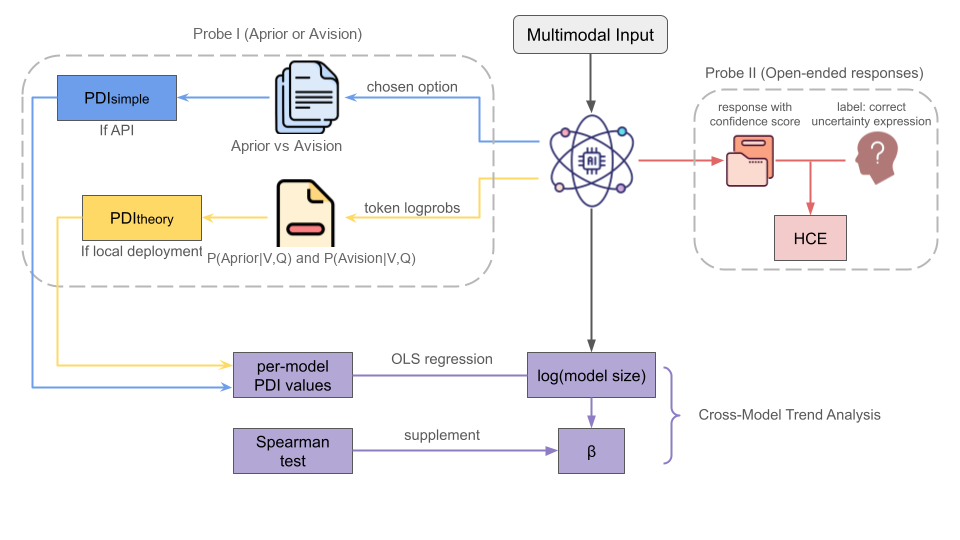
\includegraphics[width=0.9\textwidth]{howmetricswork.png}
\caption{Metric computation flow in VH-Probe. Probe~I maps temporally
reversed videos to forced-choice responses, from which
$\PDI_{\mathrm{simple}}$ is computed as the rate of language-prior-consistent
selections; for local models with token log-probabilities,
$\PDI_{\mathrm{theory}}$ is computed as the log-probability ratio between
the language-prior-consistent and visually grounded answers. Probe~II maps
masked or intrinsically ambiguous videos to open-ended responses and
confidence scores, from which $\HCE$ is computed using confidence bins and
uncertainty-expression labels. Finally, model-level $\PDI$ values are
regressed against log model size to obtain the inverse-scaling coefficient
$\beta$.}
\label{fig:metricflow}
\end{figure*}

\noindent\textbf{Stage~4: Validation and Analysis.}
We validate the metrics with control videos, text-only baselines,
category-level analysis, and local-model log-probability checks.

\begin{figure*}[t]
 \centering
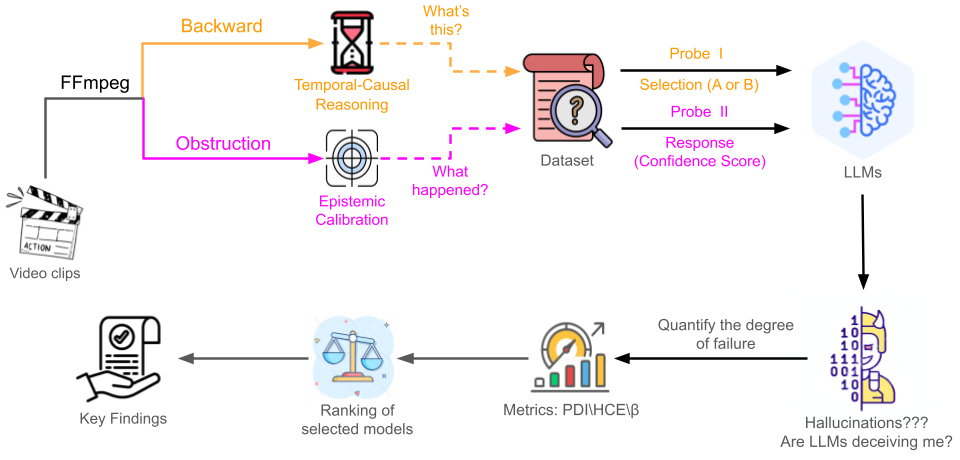
\includegraphics[width=0.9\textwidth]{Frameworkofhv.png}
 \caption{The VH-Probe evaluation pipeline. Raw video clips are
 transformed by ffmpeg into two diagnostic branches:
 Probe~I (orange, temporal reversal) elicits forced-choice selections
 scored by $\PDI$; Probe~II (pink, visual obstruction) elicits
 open-ended responses with confidence scores measured by $\HCE$.
 The Inverse Scaling Coefficient $\beta$ is fitted across models, and the
 results are examined with control videos, text-only baselines, and
 category-level analysis.}
 \label{fig:overview}
\end{figure*}


\section{Experiments}
\label{sec:exp}
%% =====================================================================

\subsection{Evaluated Models}

We evaluate six Video-LLMs that span a broad range of model capacities
and access modalities, as detailed in Table~\ref{tab:models}. The
selection is governed by two criteria. First, scale coverage:
the six models provide five distinct points on the parameter-count
axis (2B, 7B, ${\sim}$10B, 26B, ${\sim}$200B), allowing us to estimate
the inverse scaling coefficient~$\beta$ and to compute a rank-based
Spearman correlation as a descriptive trend test.
Second, access diversity: four models (Qwen2-VL-2B,
LLaVA-1.6-7B, Qwen2-VL-7B, and InternVL2-26B) are deployed locally
with 4-bit NormalFloat (NF4) quantisation, enabling computation of the theoretical
$\PDI$ from token log-probabilities; the remaining two
(Gemini~1.5~Flash and GPT-4o) are accessed via commercial APIs, for
which only the simplified forced-choice $\PDI$ is available.

Importantly, the six models originate from different architectural
families, training corpora, and alignment procedures; observed PDI
differences therefore cannot be attributed to model scale alone. We
include a within-family comparison---Qwen2-VL at 2B and 7B---to
partially isolate the scale effect from architectural confounds, but
acknowledge that a full same-family scale ladder (e.g.\
Qwen2-VL 2B/7B/72B) remains necessary for definitive causal claims
(see Section~\ref{sec:discussion}).
For the API models, GPT-4o serves here as a high-capability frontier
API baseline, while Gemini~1.5~Flash serves as a compute-efficient API
baseline. Together, the six models allow
us to assess whether the inverse scaling trend is robust across
diverse architectures.

\begin{table}[t]
\centering
\small
\caption{Models evaluated in VH-Probe. ``Both'' = simplified and
theoretical PDI reported; ``Simple'' = forced-choice rate only.
Ordinal ranking for Spearman test is based on model size; see text for
details.}
\label{tab:models}
\begin{tabular}{llll}
\toprule
\textbf{Model} & \textbf{Size} & \textbf{Access} & \textbf{PDI} \\
\midrule
Qwen2-VL-2B  & 2B   & Local 4-bit & Both \\
LLaVA-1.6-7B  & 7B   & Local 4-bit & Both \\
Qwen2-VL-7B  & 7B   & Local 4-bit & Both \\
Gemini 1.5 Flash & undisclosed* & API   & Simple \\
InternVL2-26B  & 26B   & Local 4-bit & Both \\
GPT-4o    & undisclosed* & API   & Simple \\
\bottomrule
\multicolumn{4}{l}{\scriptsize *OLS plots use community estimates
(${\sim}$10B, ${\sim}$200B) for axis positioning only;}\\
\multicolumn{4}{l}{\scriptsize \phantom{*}all statistical conclusions
rely on rank-order tests that do not require these values.}
\end{tabular}
\end{table}

\subsection{Evaluation Protocol}

Probe~I presents each long video through a length-dependent set of
two-alternative forced-choice questions. Before model evaluation, GPT-5.5
is provided with each question, its candidate answers, and the benchmark
reference description. It labels the answer favoured by ordinary-world
language knowledge as $\Aprior$ and the answer supported by the transformed
video as $\Avision$. These semantic labels are frozen and shared across all
six evaluated models. The two-alternative forced-choice format is used to
eliminate hedged or abstaining responses and to produce a single binary
signal per item for $\PDI$ computation. Probe~II pairs each long video
with a length-dependent set of open-ended uncertainty-elicitation questions
and a 0--10 confidence rating. The exact formats for both probes appear in
Section~\ref{sec:prompt_examples}.

\subsubsection{Refusal Rate Monitoring}
If a model refuses $>$20\% of prompts the template is revised to remove
safety triggers without altering diagnostic intent.

\subsection{Implementation Details}

All temporal reversals are pre-generated offline. We use YOLOv8
\cite{jocher2023yolo} to determine masking coordinates on the first frame for
clips whose target object remains spatially stable over the queried interval.
Local models run on a single NVIDIA RTX~3090 with BitsAndBytes-style
quantisation \cite{dettmers2022gpt3}. API calls use temperature~0.

\subsection{Validation Protocol}

Prior to reporting results we conduct three sanity checks:
(i)~manual inspection of 20 random long videos confirms that the
diagnostic perturbations remain perceptually unambiguous;
(ii)~model accuracy $>$79\% on unperturbed control videos confirms
baseline visual perception;
(iii)~video-level Pearson~$r$ between $\PDI_{\mathrm{simple}}$ and
$\PDI_{\mathrm{theory}}$ on local models $>0.85$.
Reported $p$-values are model-level descriptive statistics over the six
evaluated systems. Figure~\ref{fig:inversescaling} uses a video-level
cluster bootstrap for model PDI estimates, while
Figure~\ref{fig:calibration} uses Wilson intervals for the observed
uncertainty-expression proportion within each confidence bin.

%% =====================================================================
\section{Results}
\label{sec:results}
%% =====================================================================

\subsection{Probe I: Prior Dominance Index}
\label{sec:result_pdi}

%% ---- FIGURE: PDI and IPV-Bench comparison -------------------------
\begin{figure*}[t]
 \centering
 \begin{subfigure}[t]{0.49\textwidth}
  \centering
  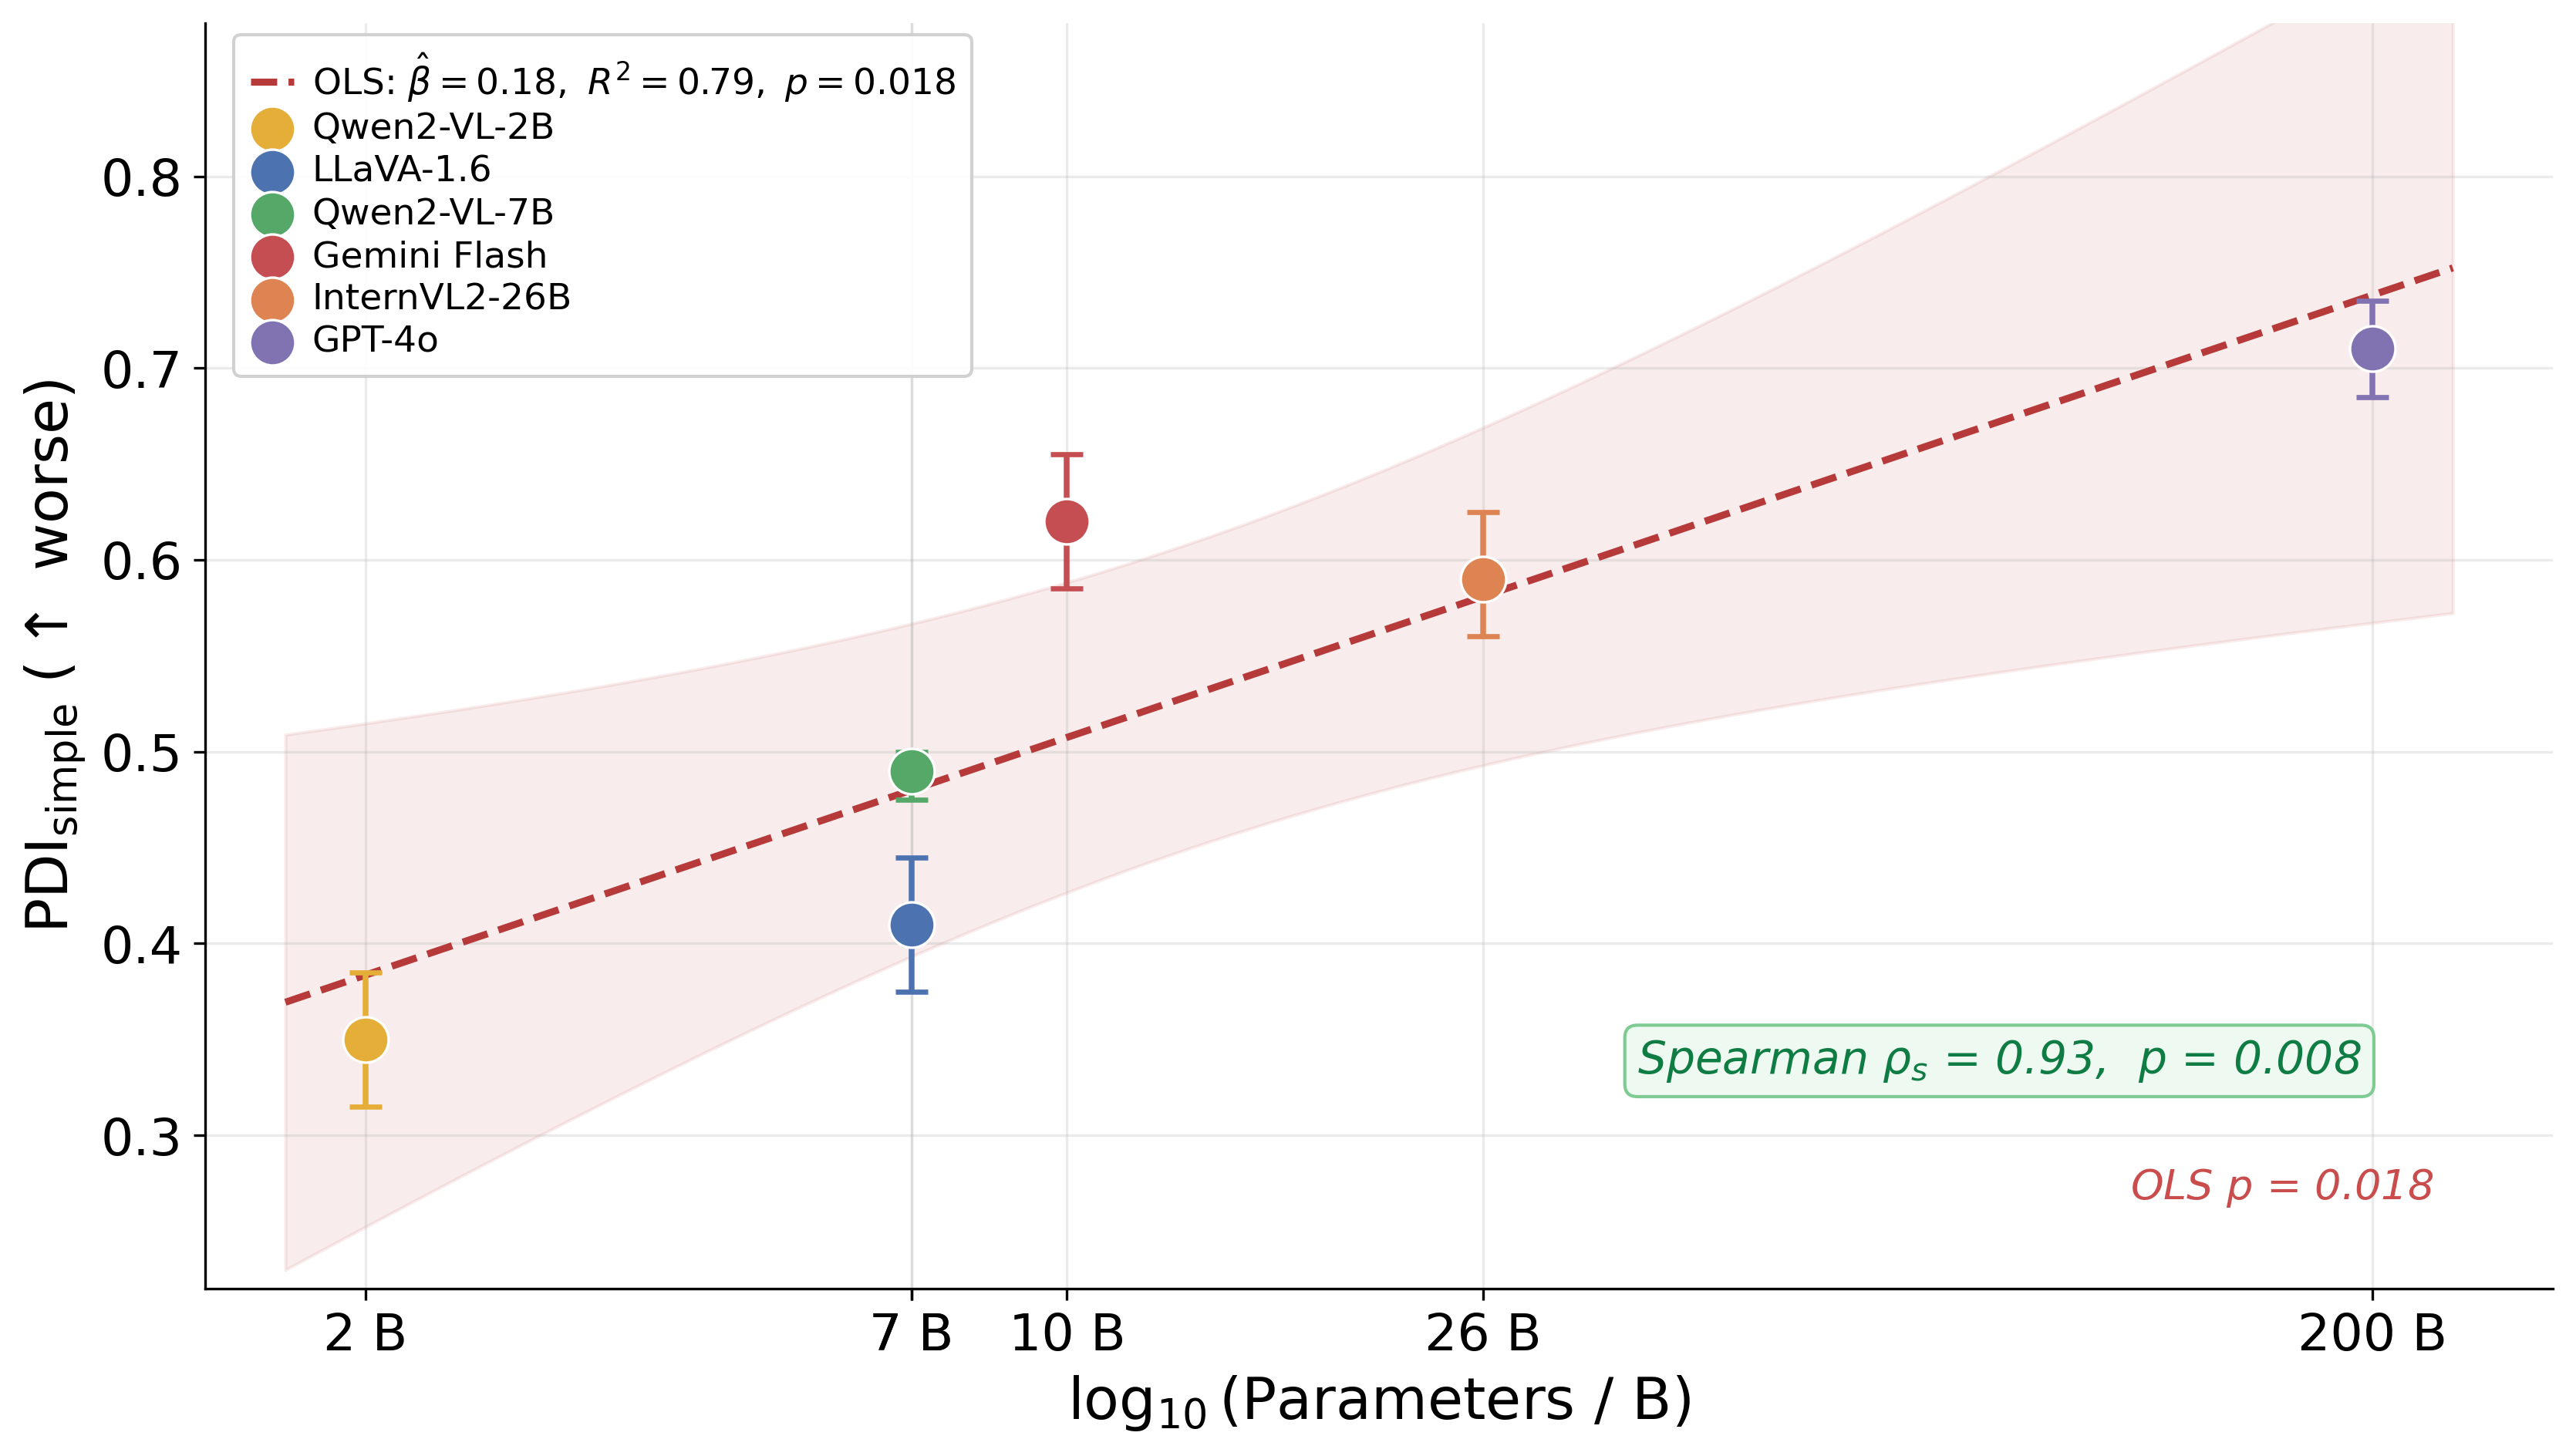
\includegraphics[width=\linewidth]{probe_i_a_inverse_scaling.png}
  \caption{$\PDI_{\mathrm{simple}}$ as a function of log model size.
  The OLS line has a positive slope ($\hat{\beta}=+0.18$,
  $R^2=0.79$). Point error bars are 95\% video-level cluster-bootstrap
  confidence intervals; the shaded region is the 95\% confidence interval
  for the mean OLS response.}
  \label{fig:inversescaling}
 \end{subfigure}
 \hfill
 \begin{subfigure}[t]{0.49\textwidth}
  \centering
  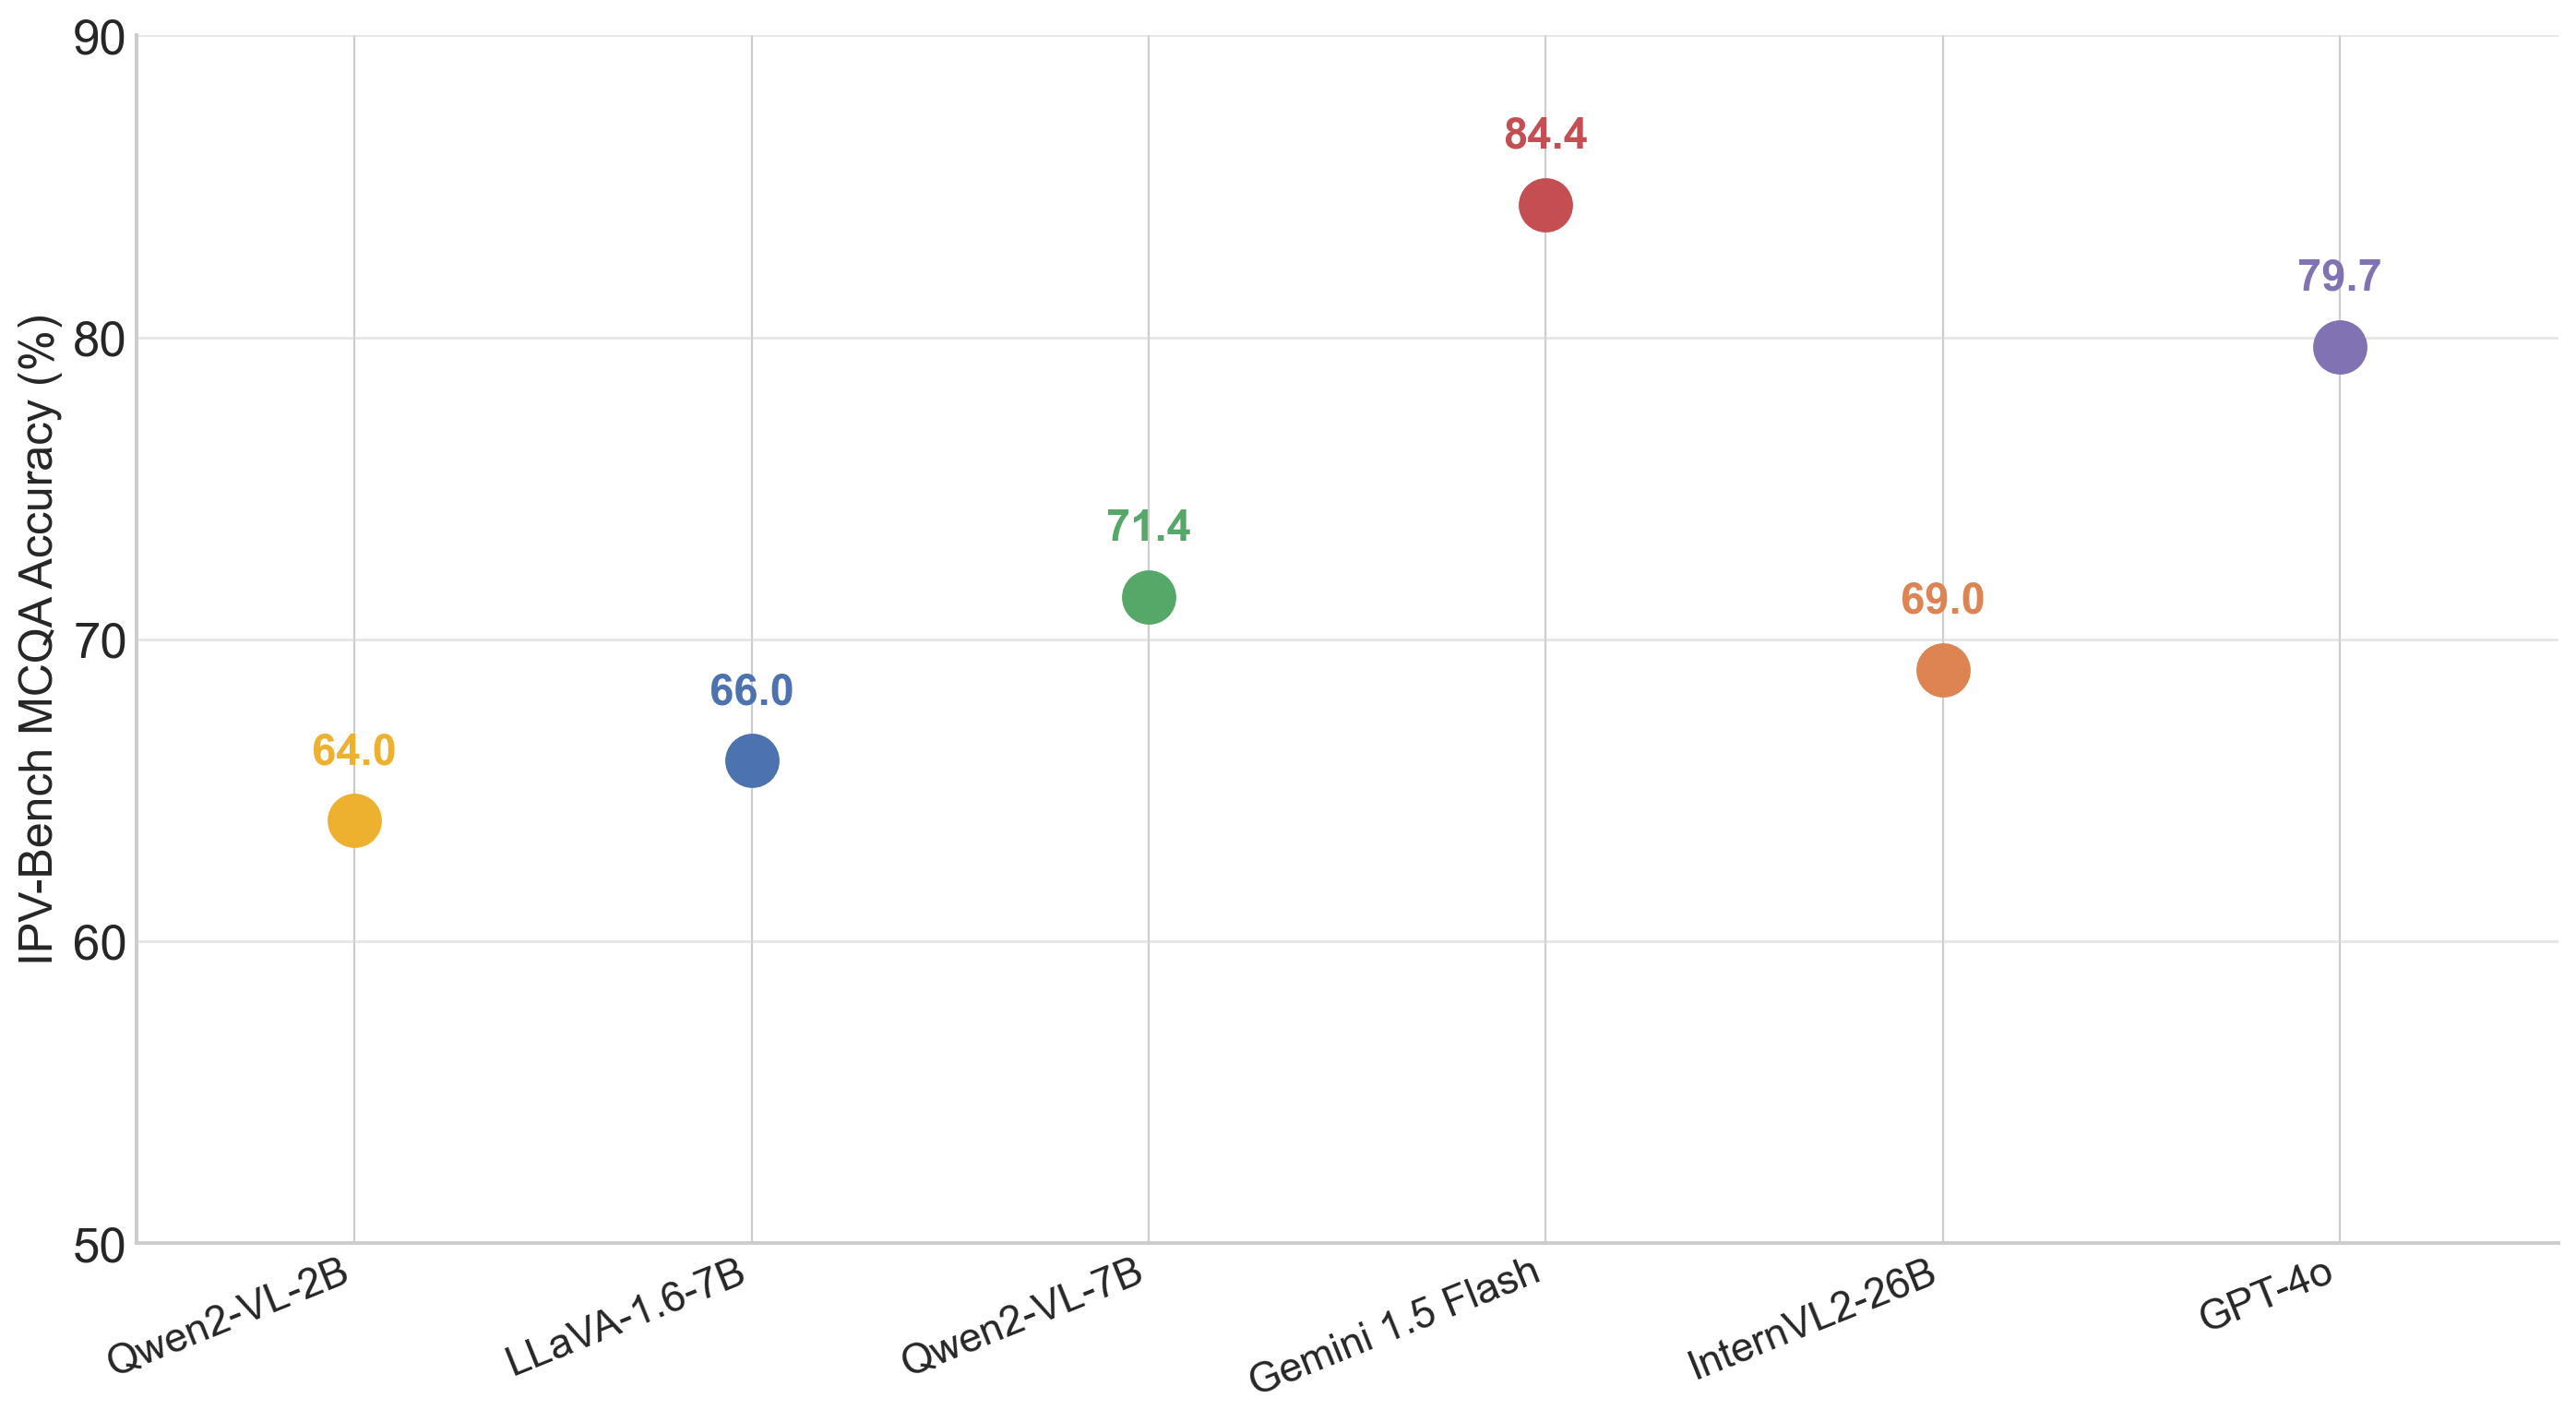
\includegraphics[width=\linewidth]{ipv_bench_mcqa_projected.png}
  \caption{IPV-Bench MCQA evaluation~\cite{bai2025impossible}, where
  higher accuracy indicates stronger multiple-choice understanding of
  impossible videos.}
  \label{fig:ipvbench-mcqa}
 \end{subfigure}
 \caption{Complementary evaluation of impossible-video understanding.
 Panel~(a) measures language prior dominance when visual evidence
 contradicts ordinary event expectations, whereas Panel~(b) reports the
 IPV-Bench MCQA evaluation. High MCQA accuracy does not necessarily imply
 low language prior dominance.}
 \label{fig:pdi-ipv-comparison}
\end{figure*}

%% ---- FIGURE: Original vs reversed accuracy drop --------------------
\begin{figure}[t]
 \centering
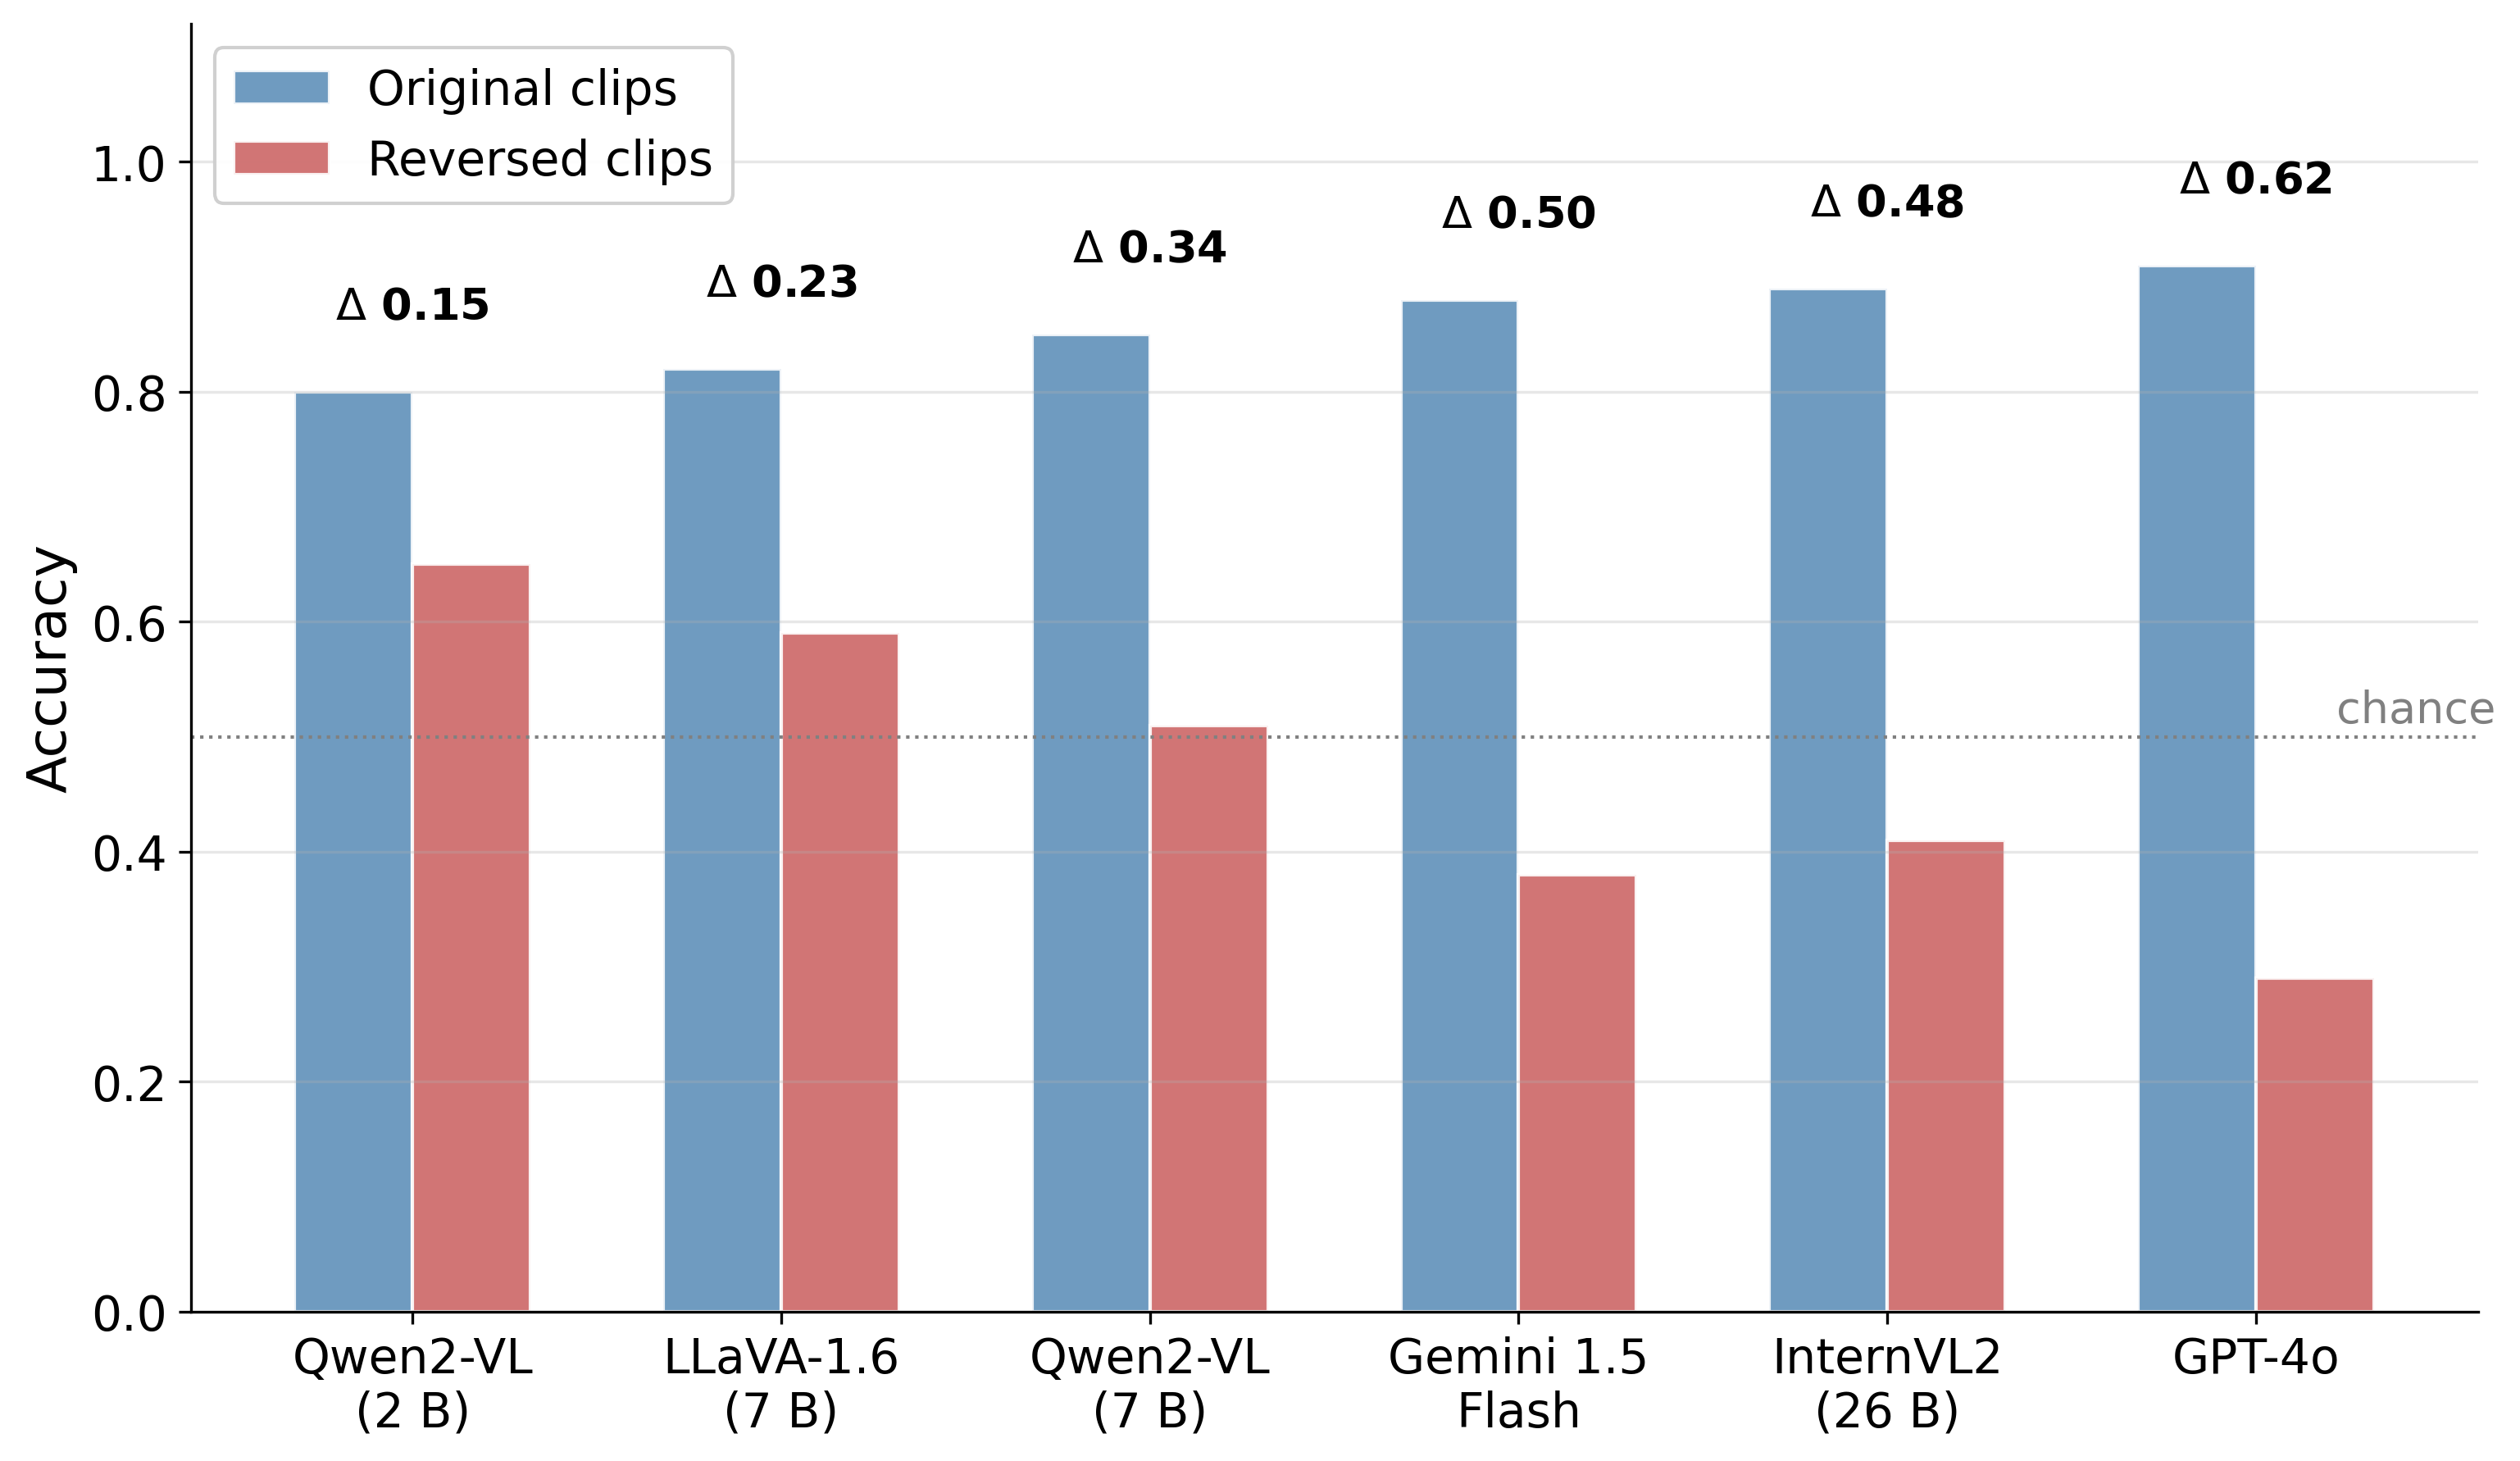
\includegraphics[width=\linewidth]{probe_i_b_accuracy_drop.png}
 \caption{Per-model accuracy on original (blue) and temporally
 reversed (red) long-form clips (Probe~I-A). All models achieve
 $>$79\% on original clips, suggesting functional visual perception;
 accuracy drops on reversed clips as models fall back on
 language priors. The accuracy gap $\Delta$ grows from 0.15
 (Qwen2-VL-2B) to 0.62 (GPT-4o).}
 \label{fig:accuracydrop}
\end{figure}

Table~\ref{tab:main_results} reports all diagnostic metrics.
Figures~\ref{fig:inversescaling}, \ref{fig:accuracydrop}, and
\ref{fig:textonly} collectively establish three findings.

\textbf{Finding 1: inverse scaling trend.}
Figure~\ref{fig:inversescaling} shows that $\PDI_{\mathrm{simple}}$
rises from 0.35 (Qwen2-VL-2B) to 0.71 (GPT-4o) as model capacity
increases. We report two complementary statistics:

\noindent Parameter-dependent (OLS):
$\hat{\beta}=+0.18$ ($R^2=0.79$, $p=0.018$, $n=6$).
The regression is statistically significant at $\alpha=0.05$ under this
six-model specification, but should be interpreted as descriptive rather
than causal because model family and training data vary across systems.
The exact $\hat{\beta}$ value also depends on community-estimated
parameter counts for the two API models.

\noindent Parameter-free (Spearman):
$\rho_s=0.93$ ($p=0.008$).
This test uses only ordinal capacity ranking
(Qwen2-VL-2B $<$ LLaVA-1.6-7B $=$ Qwen2-VL-7B $<$ Gemini $<$
InternVL2-26B $<$ GPT-4o) and is therefore less sensitive to
parameter-count uncertainty than the OLS fit.
The high rank correlation, combined with the within-family
increase from Qwen2-VL-2B (0.35) to Qwen2-VL-7B (0.49), supports an
inverse-scaling trend, although the small number of model families
prevents a causal attribution to scale alone. The minor rank swap between
InternVL2-26B (0.59) and Gemini~Flash (0.62) likely reflects architectural
differences rather than a scale reversal.

The comparison in Figure~\ref{fig:pdi-ipv-comparison} separates performance
on the IPV-Bench MCQA evaluation from resistance to language prior dominance.
Gemini~1.5~Flash and GPT-4o achieve relatively high MCQA accuracy in
Panel~(b), while also exhibiting
comparatively high $\PDI_{\mathrm{simple}}$ values in Panel~(a). This
contrast indicates that strong performance on broad impossible-video
understanding does not necessarily ensure that a model will follow visual
evidence when it directly conflicts with ordinary event expectations.


\textbf{Finding 2: collapse on reversed clips.}
Figure~\ref{fig:accuracydrop} shows that the accuracy penalty for
temporal reversal is not uniform. LLaVA-1.6-7B, one of the smaller models,
loses 23 percentage points (82\%$\to$59\%), remaining comfortably
above chance. GPT-4o, the largest, loses 62 points (91\%$\to$29\%),
falling below the 50\% chance level on a forced-choice task,
meaning it answers the reversed long-form question worse than
random under this forced-choice construction. This pattern suggests that
language-prior pressure can override the visual signal available in the
forced-choice setting.

%% ---- FIGURE: Text-only baseline ----------------------------------
\begin{figure}[t]
 \centering
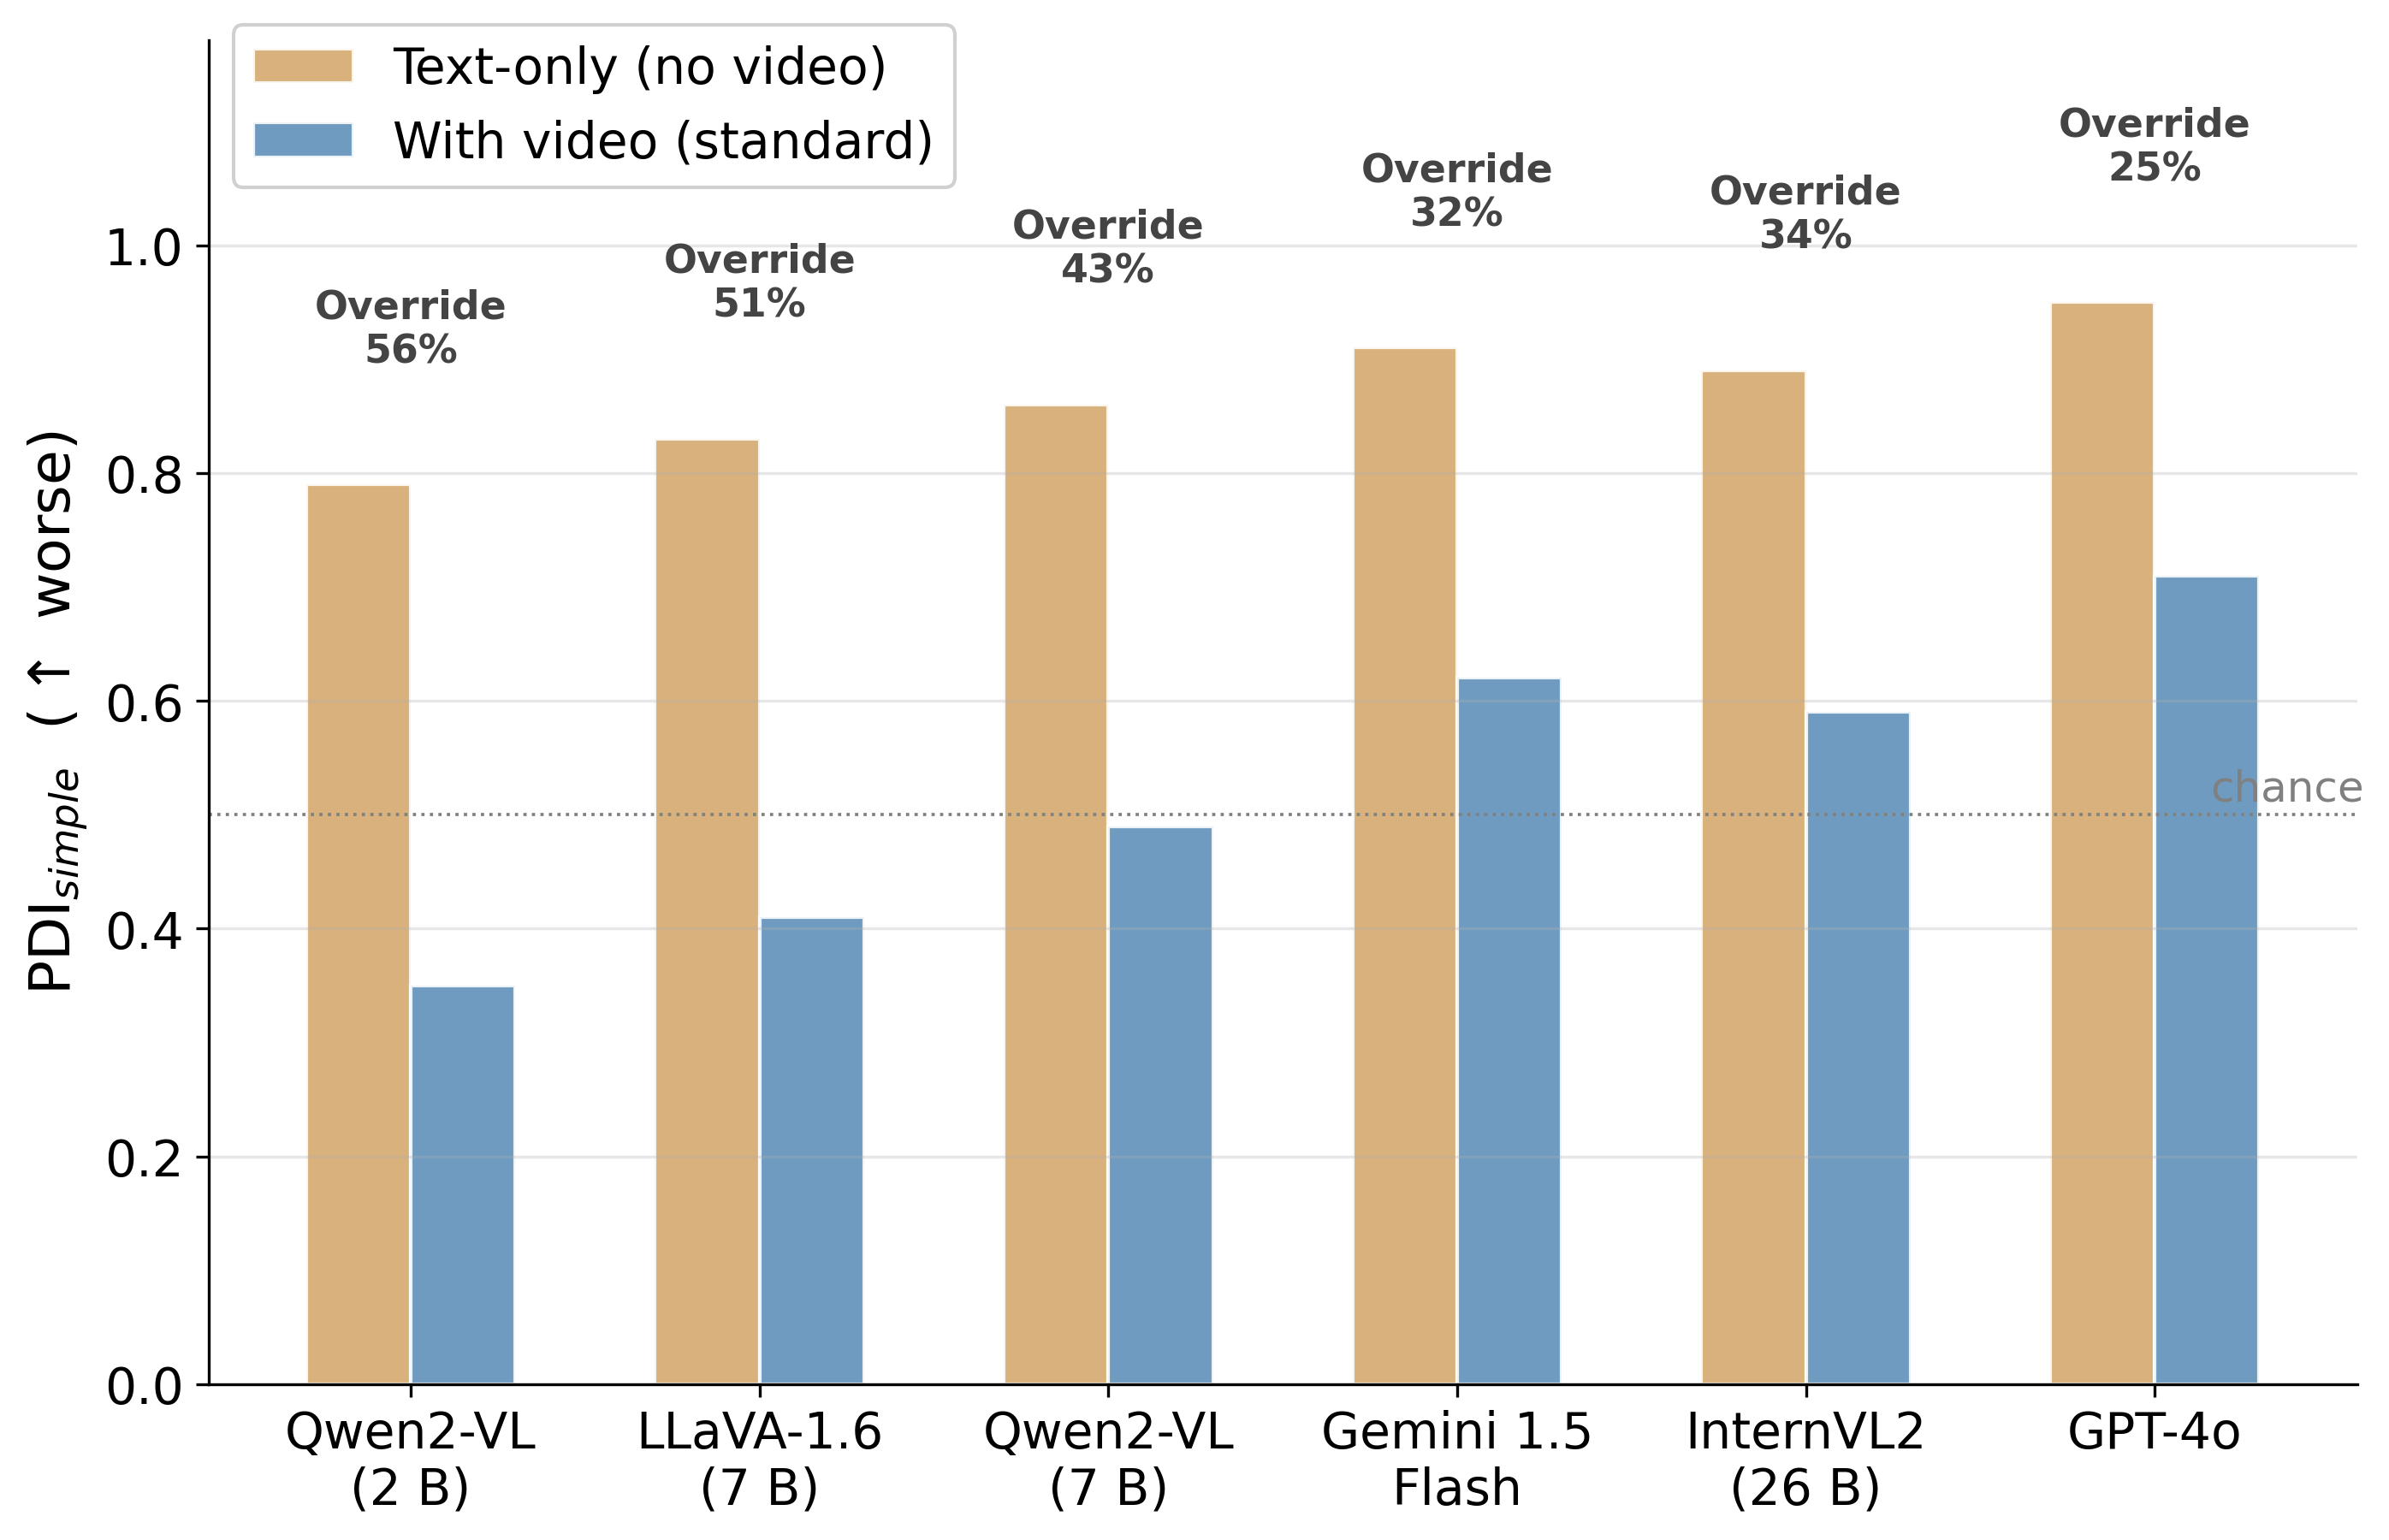
\includegraphics[width=1.05\linewidth]{fig_text_only_baseline.png}
 \caption{Text-only vs.\ visual PDI (Probe~I-A). When video input
 is withheld, all models default to language priors at rates 0.79--0.95.
 The visual override ratio (fraction of language prior dominance corrected
 by visual evidence) decreases from 56\% (Qwen2-VL-2B) to
 25\% (GPT-4o), suggesting weaker visual override in larger models on
 this probe.}
 \label{fig:textonly}
\end{figure}

\noindent\textbf{Finding 3: text-only baseline probes visual override.}
To disentangle visual perception failure from language prior dominance, we
run an additional text-only condition: each Probe~I-A question is
presented without the video.
Figure~\ref{fig:textonly} shows that text-only PDI is uniformly high
(0.79--0.95), showing that language priors alone strongly favour
$\Aprior$. Crucially, the visual override ratio---the fraction
of language prior dominance that is corrected when the video is provided---
decreases from 56\% (Qwen2-VL-2B) to 25\% (GPT-4o). This shrinkage
is consistent with the inverse scaling trend reflecting a visual-evidence
integration failure rather than perception alone: all models receive the same
video input, but larger models more often select the language-prior-consistent answer.

\begin{table}[t]
\centering
\small
\setlength{\tabcolsep}{3pt}
\caption{VH-Probe full diagnostic results.
$\PDI_s$: simplified PDI (forced-choice rate, $\downarrow$ better).
$\PDI_t$: theoretical PDI (log-prob ratio, local models only, $\downarrow$ better).
$r$: video-level Pearson correlation between $\PDI_s$ and $\PDI_t$.
$\HCE_A$/$\HCE_B$: Hallucination Calibration Error on Probe~II-A/II-B ($\downarrow$ better).}
\label{tab:main_results}
\begin{tabular}{@{}lccccc@{}}
\toprule
\textbf{Model} &
\textbf{$\PDI_s$} &
\textbf{$\PDI_t$} &
\textbf{$r$} &
\textbf{$\HCE_A$} &
\textbf{$\HCE_B$} \\
\midrule
Qwen2-VL-2B      & 0.35 & 0.33 & 0.88 & 0.18 & 0.10 \\
LLaVA-1.6-7B     & 0.41 & 0.39 & 0.87 & 0.22 & 0.14 \\
Qwen2-VL-7B      & 0.49 & 0.47 & 0.89 & 0.30 & 0.25 \\
Gemini 1.5 Flash & 0.62 & \textit{n/a} & \textit{n/a} & 0.37 & 0.22 \\
InternVL2-26B    & 0.59 & 0.57 & 0.91 & 0.33 & 0.28 \\
GPT-4o           & 0.71 & \textit{n/a} & \textit{n/a} & 0.42 & 0.35 \\
\midrule
\multicolumn{6}{@{}l@{}}{\footnotesize\textit{n/a}: log-probabilities inaccessible via API.} \\
\multicolumn{6}{@{}l@{}}{\footnotesize OLS: $\hat{\beta}=+0.18$, $R^2=0.79$, $p=0.018$; Spearman $\rho_s=0.93$, $p=0.008$.} \\
\bottomrule
\end{tabular}
\end{table}




\subsubsection{Simplified vs.\ Theoretical PDI}
For each local model, the Pearson~$r$ between video-level
$\PDI_{\mathrm{simple}}$ and $\PDI_{\mathrm{theory}}$ scores is reported
in Table~\ref{tab:main_results}.
Strong correlation ($r>0.85$) validates the API-compatible simplified
metric as a faithful proxy.

\subsection{Probe II: Epistemic Overconfidence}
\label{sec:result_hce}

%% ---- FIGURE 6: Reliability diagram ---------------------------------
\begin{figure}[t]
 \centering
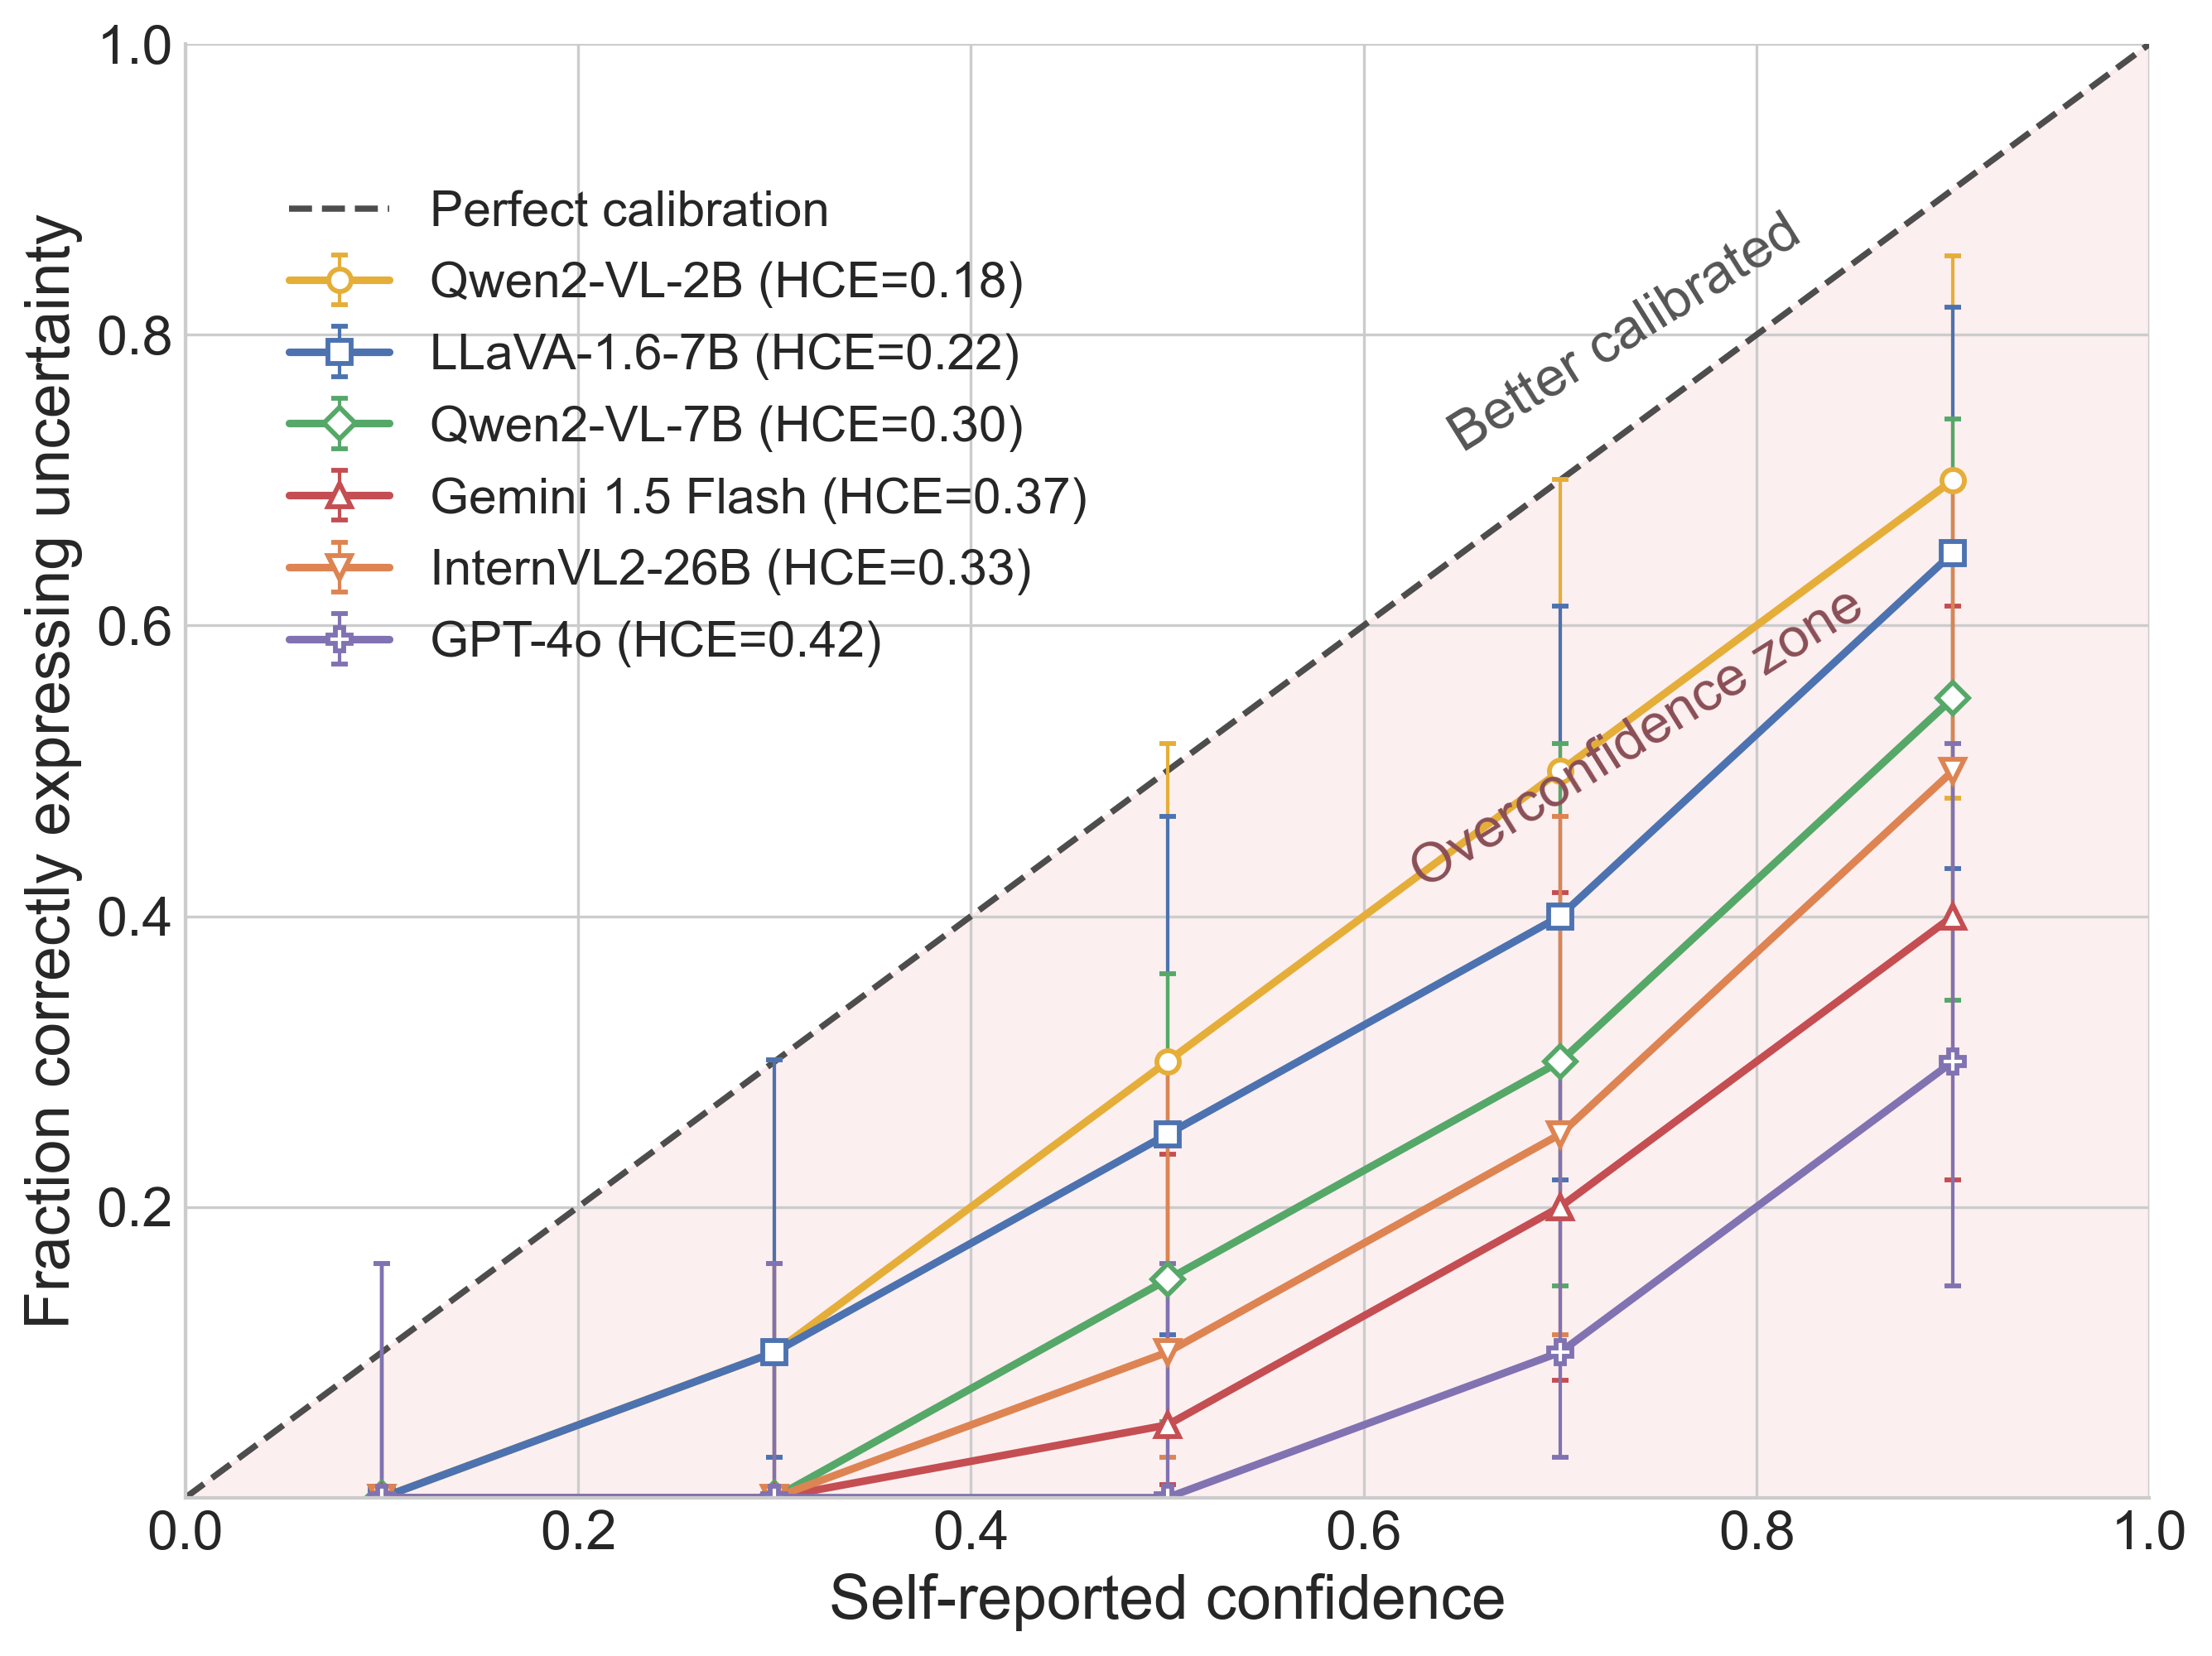
\includegraphics[width=\linewidth]{probe_ii_a_reliability.png}
\caption{Binned reliability profiles for Probe~II-A (externally masked evidence).
 The dashed diagonal represents perfect calibration ($y=x$).
 All evaluated models deviate toward the lower-right quadrant
 (high self-reported confidence, low fraction of correct uncertainty
 expressions), suggesting systematic epistemic overconfidence.
 HCE values are annotated per model in the legend. Error bars are 95\%
 Wilson confidence intervals over the observed responses in each
 confidence bin.}
 \label{fig:calibration}
\end{figure}

Figure~\ref{fig:calibration} presents the reliability diagram for
Probe~II-A. All six model curves lie below the $y=x$ diagonal, indicating
poor calibration under missing evidence. The HCE annotations show that
Qwen2-VL-2B ($\HCE=0.18$) is closest to the diagonal, while GPT-4o
($\HCE=0.42$) is furthest from it. This pattern mirrors the inverse scaling
trend observed for $\PDI$: in this probe, larger and more capable models
appear more epistemically overconfident.

The divergence between curves is most pronounced at the high-confidence
end of the x-axis, where larger models remain substantially more
confident than warranted by their uncertainty-expression accuracy.
Smaller local models remain closer to the calibration diagonal, but no
model approaches the ideal $y=x$ line. This pattern is consistent with
the possibility that helpfulness-oriented alignment discourages
abstention under missing evidence.

Table~\ref{tab:hce_intphys} provides a complementary view with the
controlled Probe~II-B (intrinsically ambiguous events) results. Across the
six evaluated models, task accuracy remains near chance level, yet
self-reported confidence exceeds observed accuracy in every case. The
resulting positive aggregate confidence gaps indicate overconfidence under
this forced-choice construction, while the 50\% chance level serves only as
a random-guessing baseline. These results therefore suggest that epistemic
miscalibration persists even when the task is designed to be maximally
ambiguous.

\begin{table}[t]
\centering
\small
\caption{Accuracy vs.\ self-reported confidence for intrinsically ambiguous events (Probe~II-B).
 Excess confidence = Avg.\ Confidence $-$ Accuracy.
 Positive values indicate that aggregate self-reported confidence exceeds
 observed accuracy under this forced-choice construction.}
\label{tab:hce_intphys}
\begin{tabular}{lrrr}
\toprule
\textbf{Model} & \textbf{Acc.} & \textbf{Avg.\ Conf.} & \textbf{Excess} \\
\midrule
Qwen2-VL-2B      & 50\% & 60\% & +10\%\\
LLaVA-1.6-7B  & 51\% & 65\% & +14\% \\
Qwen2-VL-7B  & 49\% & 70\% & +21\% \\
Gemini 1.5 Flash & 52\% & 76\% & +24\% \\
InternVL2-26B    & 49\% & 77\% & +28\% \\
GPT-4o   & 48\% & 83\% & +35\% \\
\bottomrule
\end{tabular}
\end{table}

\subsection{Category-Level Analysis}
\label{sec:category_analysis}

%% ---- FIGURE: Per-category PDI ------------------------------------
\begin{figure}[t]
 \centering
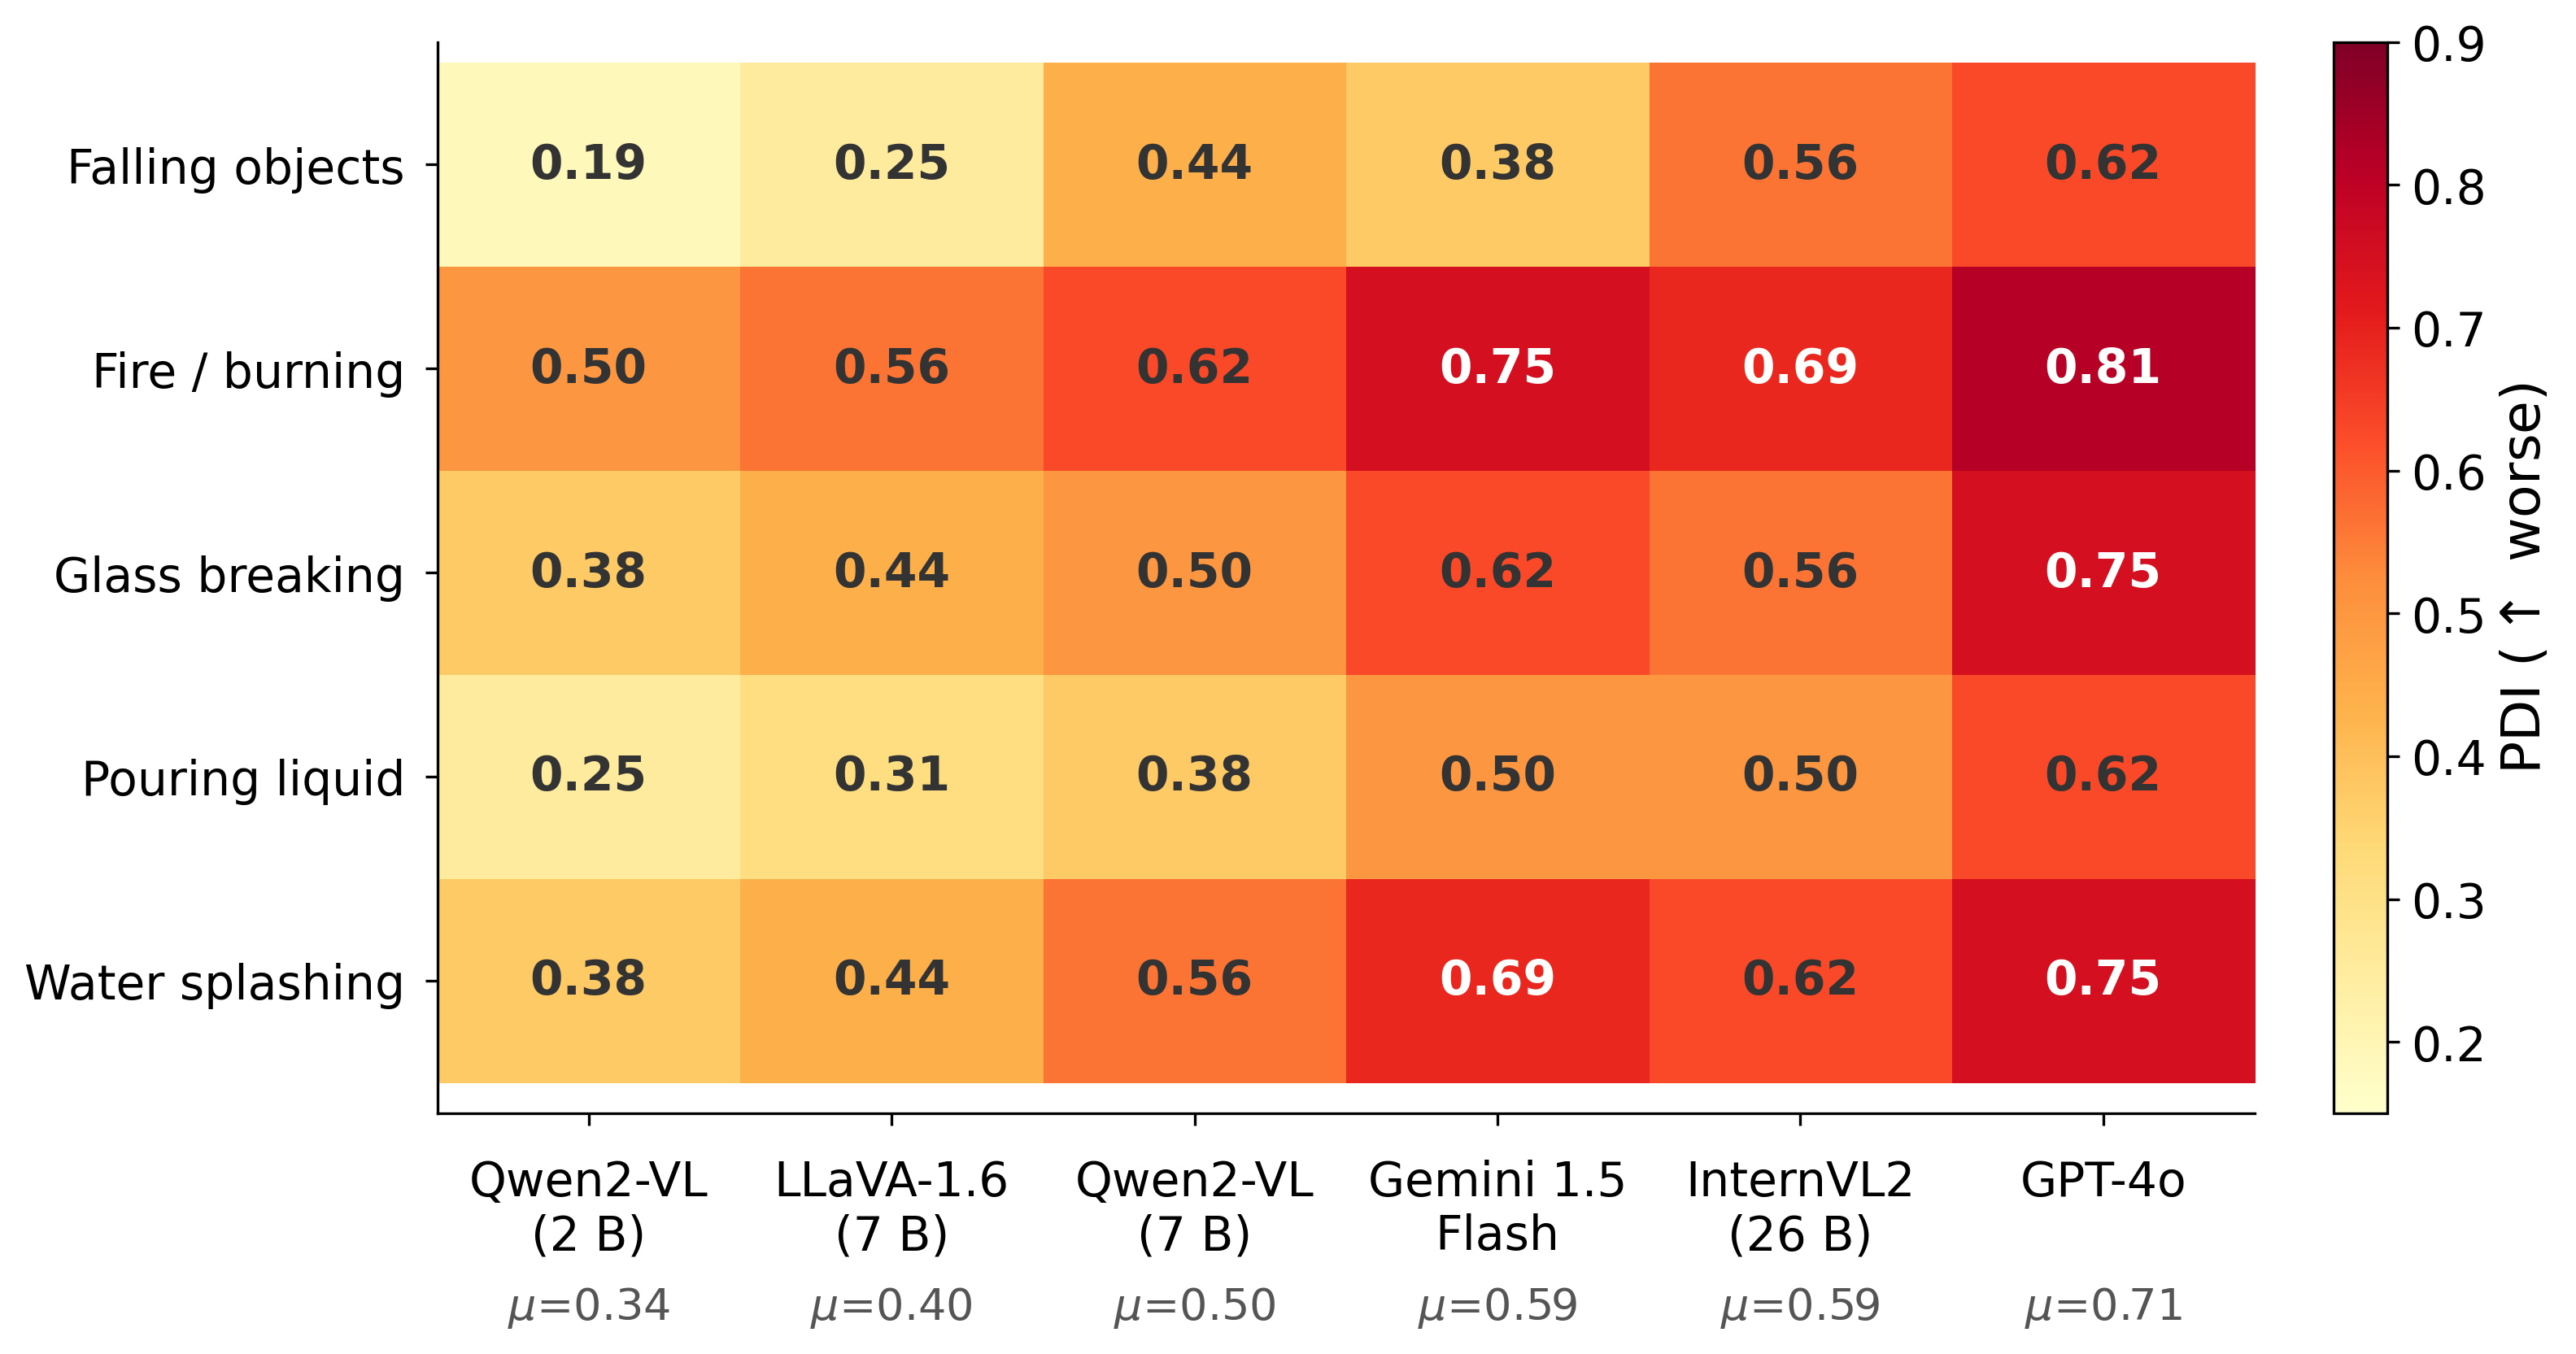
\includegraphics[width=\linewidth]{fig_per_category_pdi.png}
 \caption{Per-category $\PDI_{\mathrm{simple}}$ heatmap (Probe~I-A).
The heatmap shows an overall increase in $\PDI_{\mathrm{simple}}$
from smaller open-source models to stronger API/frontier models, while
also revealing architecture-dependent deviations such as Gemini Flash
exceeding InternVL2-26B in several categories. \textit{Fire/burning} exhibits the highest PDI across all
 models (strongest language prior), while \textit{falling objects}
 has the lowest (most visually salient reversal).}
 \label{fig:percategory}
\end{figure}

Figure~\ref{fig:percategory} provides a category-level breakdown of
$\PDI_{\mathrm{simple}}$ for Probe~I-A. The overall increase in column means is consistent with the aggregate
$\PDI_{\mathrm{simple}}$ trend in Table~\ref{tab:main_results}, indicating
that the effect is not driven by a single semantic class. Among the five categories, \textit{fire/burning} exhibits the highest
PDI across models, suggesting especially strong language-prior pull, whereas
\textit{falling objects} remains comparatively lower, consistent with
its visually salient reversal cues.


\section{Discussion}
\label{sec:discussion}
%% =====================================================================

\subsection{Interpreting Language Prior Dominance}

VH-Probe should be interpreted as a diagnostic benchmark rather than a broad
leaderboard. Its probes deliberately narrow the setting to
cases where visual evidence conflicts with language priors or where decisive
evidence is unavailable. The benchmark is therefore less comprehensive than
Video-MME, MVBench, or LongVideoBench, but it isolates a failure mode that
general video QA scores can hide.

\subsection{Why Temporal Reversal Reduces the Artefact Confound}

Reversed clips are pixel-identical to their originals on a per-frame basis;
only frame order differs. A model cannot solve Probe~I by detecting synthetic
video artefacts or frame-level distribution shifts. Instead, it must decide
whether to follow the observed temporal evidence or the more common event
described by language priors. This differs from generated impossible-video
benchmarks, where unrealistic textures, motion artefacts, or generation
failures may become confounds \cite{bai2025impossible}. Temporal
reversal is not a complete proxy for physical reasoning, but it provides a
controlled stress test for temporal-causal grounding.

\subsection{Calibration under Missing Evidence}

The Probe~I results are consistent with a shortcut-learning interpretation:
models often choose the answer that is most plausible under common event
statistics even when the video shows the reverse process. This does not imply
that larger models are globally worse at video understanding. Rather, it
suggests that stronger language priors can become a liability when the task
requires overriding ordinary-world expectations. The result therefore
complements inverse-scaling findings in text-only settings
\cite{mckenzie2023inverse,wei2023inverse,shi2023large}.

Probe~II points to a related calibration problem. Instruction-following and
RLHF-style alignment can reward helpful, complete answers
\cite{ouyang2022training}, but this objective may conflict with epistemic
humility when visual evidence is masked or intrinsically ambiguous. A
well-calibrated Video-LLM should not merely provide a fluent answer; it should
also recognise when the video does not support that answer. $\HCE$ measures
this failure mode by treating uncertainty expression as the desired behaviour
under information deprivation.

\subsection{Architecture--Scale Confound}
\label{sec:arch_confound}
The six evaluated models differ not only in parameter count but also in
architecture, training data, and alignment procedure. Consequently,
PDI differences cannot be attributed to scale alone.
Three observations partially mitigate this confound:
(1)~The two Qwen2-VL checkpoints (2B and 7B) share architecture and
training pipeline yet exhibit a clear PDI increase
($0.35 \to 0.49$), providing within-family evidence for a scale
effect.
(2)~The two architecturally distinct 7B models (LLaVA-1.6 and
Qwen2-VL) already differ in PDI ($0.41$ vs.\ $0.49$), showing
that architecture contributes; our claim is not that scale is the
sole driver, but that it is a systematic trend.
(3)~The category-level heatmap shows that the aggregate increase is not driven
by a single semantic class, even though individual categories still exhibit
model-family deviations such as the Gemini--InternVL2 reversal.
Nonetheless, a definitive isolation of the scale effect requires a
same-family scale ladder spanning at least three sizes (e.g.\
Qwen2-VL 2B/7B/72B), which we regard as an important extension of this work.

\subsection{Scale, Architecture, and Access Limitations}

Several limitations remain. First, the model sample is small: six models are
enough for an initial descriptive trend analysis, but not enough for strong
causal claims about scale independent of architecture, data, and alignment.
Second, parameter counts for Gemini~1.5~Flash and GPT-4o are undisclosed, so
the OLS estimate of $\hat{\beta}$ depends on community size estimates; the
rank-based Spearman analysis is therefore more robust than the fitted slope.
Third, forced-choice Probe~I questions make language-prior selection easy to measure
but do not capture graded explanations or partially correct reasoning. Fourth,
Probe~II focuses on English prompts and confidence self-reports, which may be
affected by model-specific calibration and instruction-following behaviour.
Finally, the masking protocol uses fixed occlusion boxes; future work should
evaluate moving masks, object-level segmentation masks, and human-annotated
uncertainty labels.


\section{Conclusion}
\label{sec:conclusion}
%% =====================================================================

We presented \textbf{VH-Probe}, a diagnostic benchmark exposing language prior
dominance and epistemic overconfidence in Video-LLMs. By relying exclusively on
deterministic transformations of public datasets, VH-Probe avoids the
generative-AI artefact confound that affects concurrent work. Our metrics
include API-friendly proxies and a theoretical variant that uses token
log-probabilities when available. Across the six evaluated video language
models, both OLS ($p=0.018$) and Spearman rank correlation ($\rho_s=0.93$,
$p=0.008$) support an inverse-scaling trend ($\hat{\beta}>0$), suggesting that
model scaling can coincide with stronger language-prior bias rather than better
visual grounding in these settings. Future Video-LLM evaluation should therefore
jointly measure visual grounding, language-prior sensitivity, and uncertainty
calibration.

\section*{Code Availability}
The implementation and evaluation scripts are available from the
\githublink.

\bibliographystyle{IEEEtran}
\bibliography{example}

\end{document}
